\documentclass{beamer}					% Document class

\usepackage[english]{babel}				% Set language
\usepackage[utf8x]{inputenc}			% Set encoding

\mode<presentation>						% Set options
{
  \usetheme{default}					% Set theme
  \usecolortheme{default} 				% Set colors
  \usefonttheme{default}  				% Set font theme
  \setbeamertemplate{caption}[numbered]	% Set caption to be numbered
}

% Uncomment this to have the outline at the beginning of each section highlighted.
%\AtBeginSection[]
%{
%  \begin{frame}{Outline}
%    \tableofcontents[currentsection]
%  \end{frame}
%}

\usepackage{graphicx}					% For including figures
\graphicspath{{figure/}}				% Shared figure folder for all labs
\usepackage{booktabs}					% For table rules
\usepackage{hyperref}					% For cross-referencing
\usepackage{subcaption}  % 記得加在 preamble
\usepackage{multicol}

\title{Introduction to R}	% Presentation title
\author{Rex Shao-Yu Wang}								% Presentation author
\institute{}					% Author affiliation
\date{September 14, 2026}									% Today's date

\begin{document}

% Title page
% This page includes the informations defined earlier including title, author/s, affiliation/s and the date
\begin{frame}
  \titlepage
\end{frame}

% Outline
% This page includes the outline (Table of content) of the presentation. All sections and subsections will appear in the outline by default.
\begin{frame}{Outline}
  \tableofcontents
\end{frame}

% The following is the most frequently used slide types in beamer
% The slide structure is as follows:
%
%\begin{frame}{<slide-title>}
%	<content>
%\end{frame}

\section{Introduction}
\begin{frame}{About Me}
  \begin{itemize}
    \item Rex Wang
    \item Second-year master's student in Agronomy Biostatistics
    \item Feel free to email me if you have any questions
    \item Email: R14621207@ntu.edu.tw
    \item Feel free to interrupt me if you have any questions
  \end{itemize}
\end{frame}

\begin{frame}{Lab Schedule}

  \begin{columns}[T]

    % Left column
    \column{0.35\textwidth}
    \textbf{Time \& Location}

    \vspace{0.5em}
    \begin{itemize}
      \item Monday 13:20--14:10
      \item Boya 408
      \item One week behind theory class
    \end{itemize}

    % Right column
    \column{0.7\textwidth}
    \textbf{Weekly Topics}

    \vspace{0.5em}

    \small
    \renewcommand{\arraystretch}{1.0}
    \begin{tabular}{lll}
      \toprule
      \textbf{Week} & \textbf{Date} & \textbf{Topic} \\
      \midrule
      1  & 9/7 & No class \\
      2  & 9/14 & Introduction to R \\
      3  & 9/21 & R Basic \\
      4  & 9/28 & No class (Holiday) \\
      5  & 10/5 & Data Type \& Transformation \\
      6  & 10/12 & Data Visualization\\
      7  & 10/19 & Probability Distribution \\
      8  & 10/26 & No class (Holiday) \\
      9  & 11/2 & No class (Midterm Exam) \\
      10 & 11/9 & Interval Estimation\\
      11 & 11/16 & Hypothesis Testing I \\
      12 & 11/23 & Hypothesis Testing II\\
      13 & 11/30 & Analysis of Variance\\
      14 & 12/7  & Correlation \& Simple Regression \\
      15 & 12/14 & Categorical Data Analysis \\
      16 & 12/21 & No class (Final Exam)  \\
      \bottomrule
    \end{tabular}
  \end{columns}
\end{frame}

\begin{frame}{Rules of Lab Session}

  \begin{columns}[T]

    % Left column
    \column{0.75\textwidth}

    \begin{itemize}
      \item No food or drink allowed!
      \item Lab Session: 20\% of total grade
    \end{itemize}

    \begin{enumerate}
      \item Participation: 5\% of total grade
      \begin{itemize}
        \item Attendance will be taken every class
        \item Calculated as: \\
        (times attended / total sessions) $\times$ 5\%
      \end{itemize}
      \item Lab Assignment: 15\% of total grade
      \begin{itemize}
        \item 4 assignments this semester
        \item Available on NTU COOL
        \item Plagiarism $\rightarrow$ 0\% for all involved
      \end{itemize}
    \end{enumerate}

    % Right column
    \column{0.35\textwidth}
    \vspace{-30pt}
    
\includegraphics[width=\textwidth]{f9eje-srjou.jpg}

  \end{columns}

\end{frame}


\section{R and R Studio}

\begin{frame}{R and RStudio}

  \begin{columns}[T]

    % Left column
    \column{0.75\textwidth}

    \small

    \textbf{R} is a programming language used for statistical computing and data visualization.

    \vspace{0.5em}

    \textbf{RStudio} is an integrated development environment (IDE) that provides a user-friendly interface for working with R.
    \begin{itemize}
      \item Free
      \item Continuous improvement (R-4.6.1 now)
      \item Low barrier to coding
      \item Available at:
      \begin{itemize}
        \item R: \url{https://cran.r-project.org/}
        \item RStudio: \url{https://posit.co/downloads}
      \end{itemize}
    \end{itemize}

    % Right column
    \column{0.35\textwidth}
    \vspace{0pt}

    \centering
    
\includegraphics[width=0.7\linewidth]{R_logo.svg.png}

    \vspace{1em}

    
\includegraphics[width=0.9\linewidth]{rstudio.png}

  \end{columns}

\end{frame}

\begin{frame}{Installation}
  \begin{enumerate}
    \item Download R from \url{https://cran.r-project.org/}
    \item Download RStudio from \url{https://posit.co/downloads}
  \end{enumerate}

  \vspace{10pt}
  \textbf{Please install R first, then RStudio.}
\end{frame}

\begin{frame}{Download R}
  \begin{figure}
    \centering
    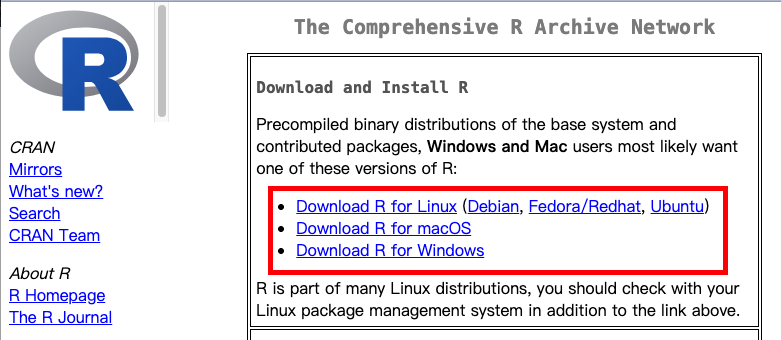
\includegraphics[width=1\linewidth]{截圖 2026-02-27 上午11.11.18.png}
  \end{figure}
\end{frame}

\begin{frame}{Download R}
  \begin{figure}
    \centering
    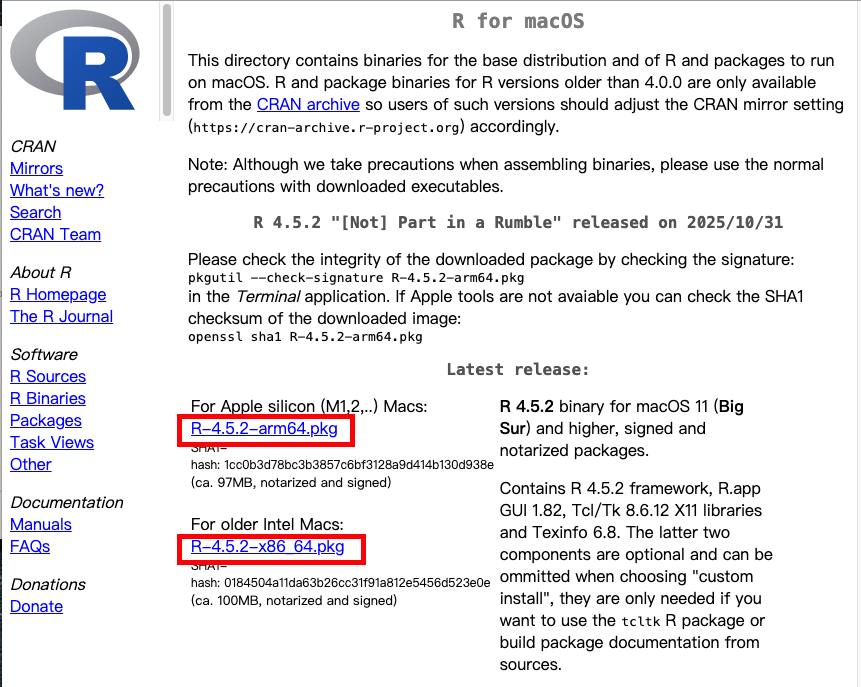
\includegraphics[width=1\linewidth]{截圖 2026-02-27 上午11.15.29.png}
  \end{figure}
\end{frame}

\begin{frame}{Download R}

  \begin{columns}[T]

    \column{0.5\textwidth}
    \centering
    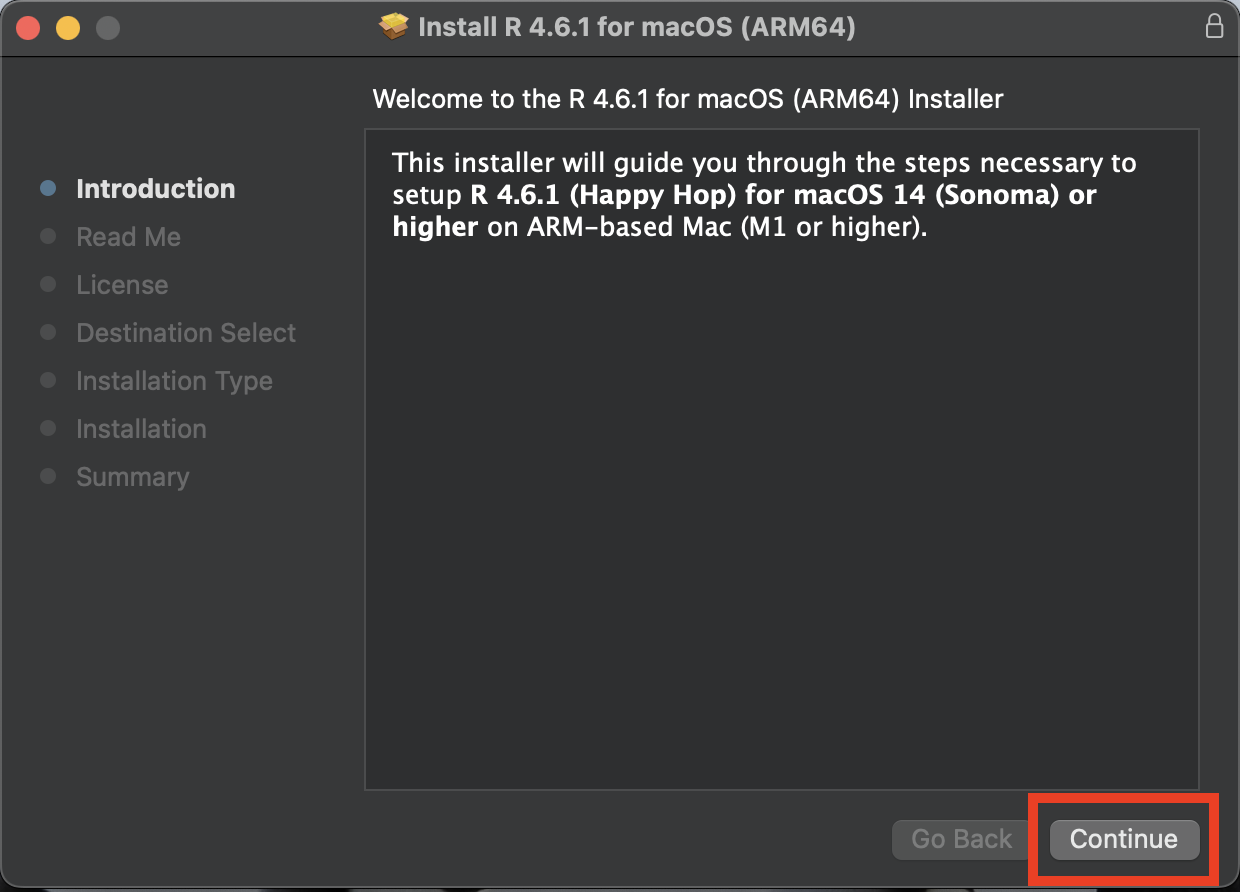
\includegraphics[width=1.1\linewidth]{R_install1.png}

    \column{0.5\textwidth}
    \centering
    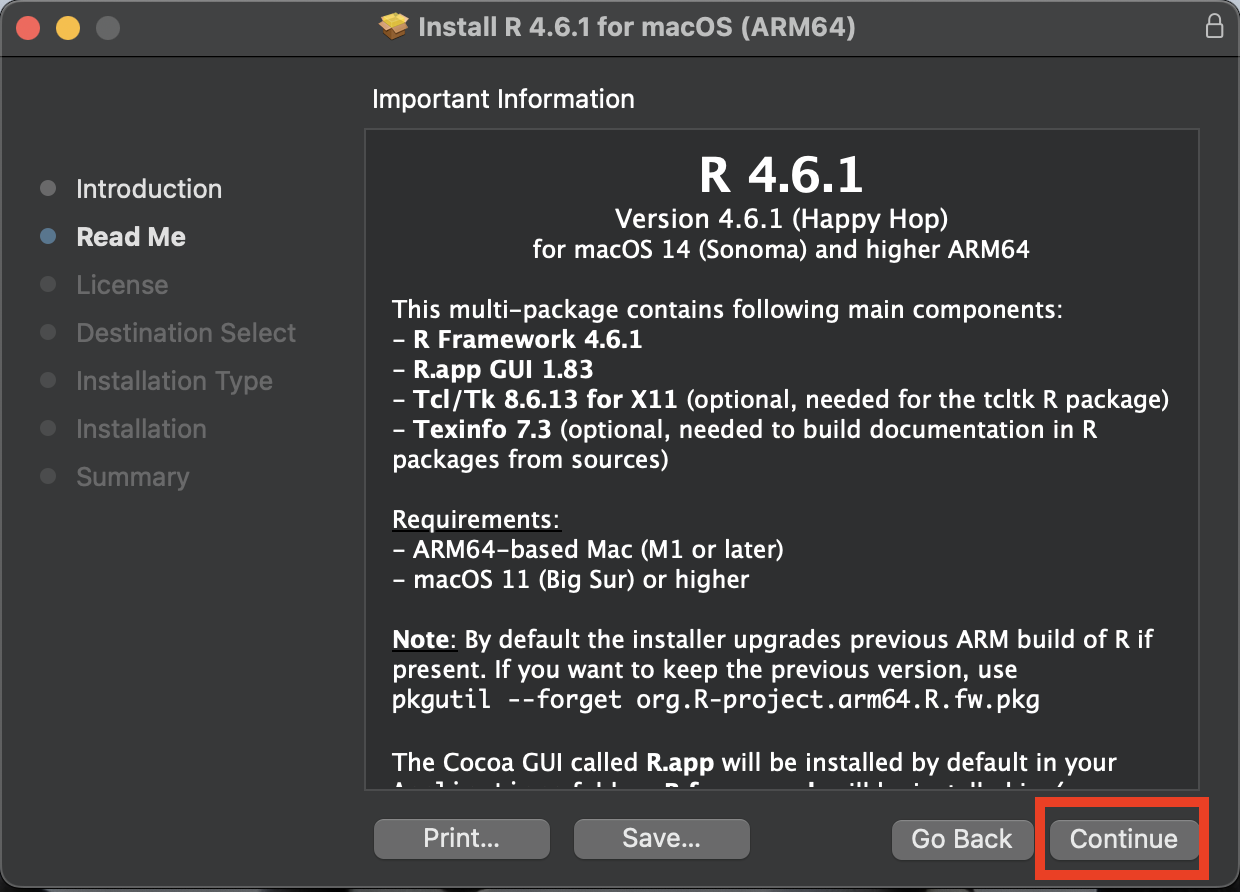
\includegraphics[width=1.1\linewidth]{R_install2.png}

  \end{columns}

\end{frame}

\begin{frame}{Download R}

  \begin{columns}[T]

    \column{0.5\textwidth}
    \centering
    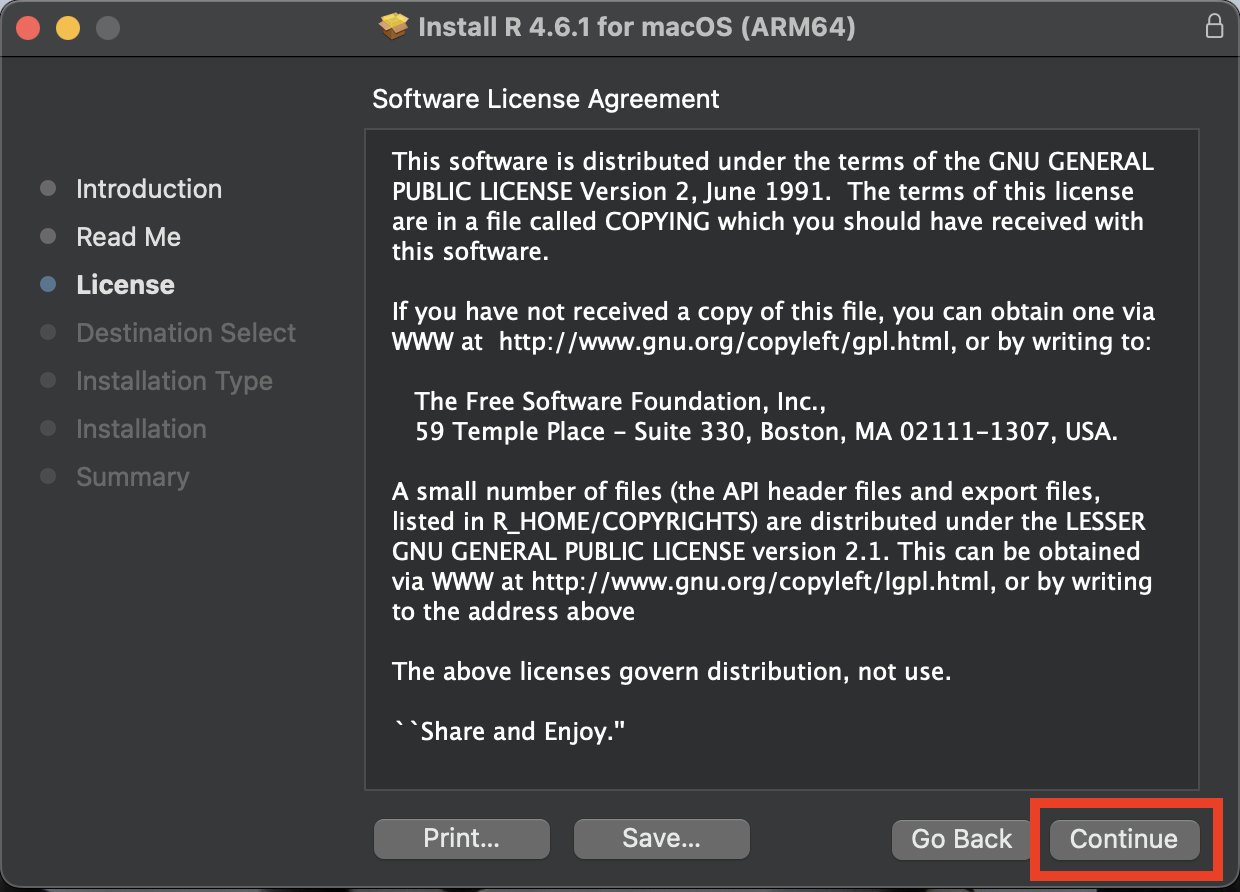
\includegraphics[width=1.1\linewidth]{R_install3.png}

    \column{0.5\textwidth}
    \centering
    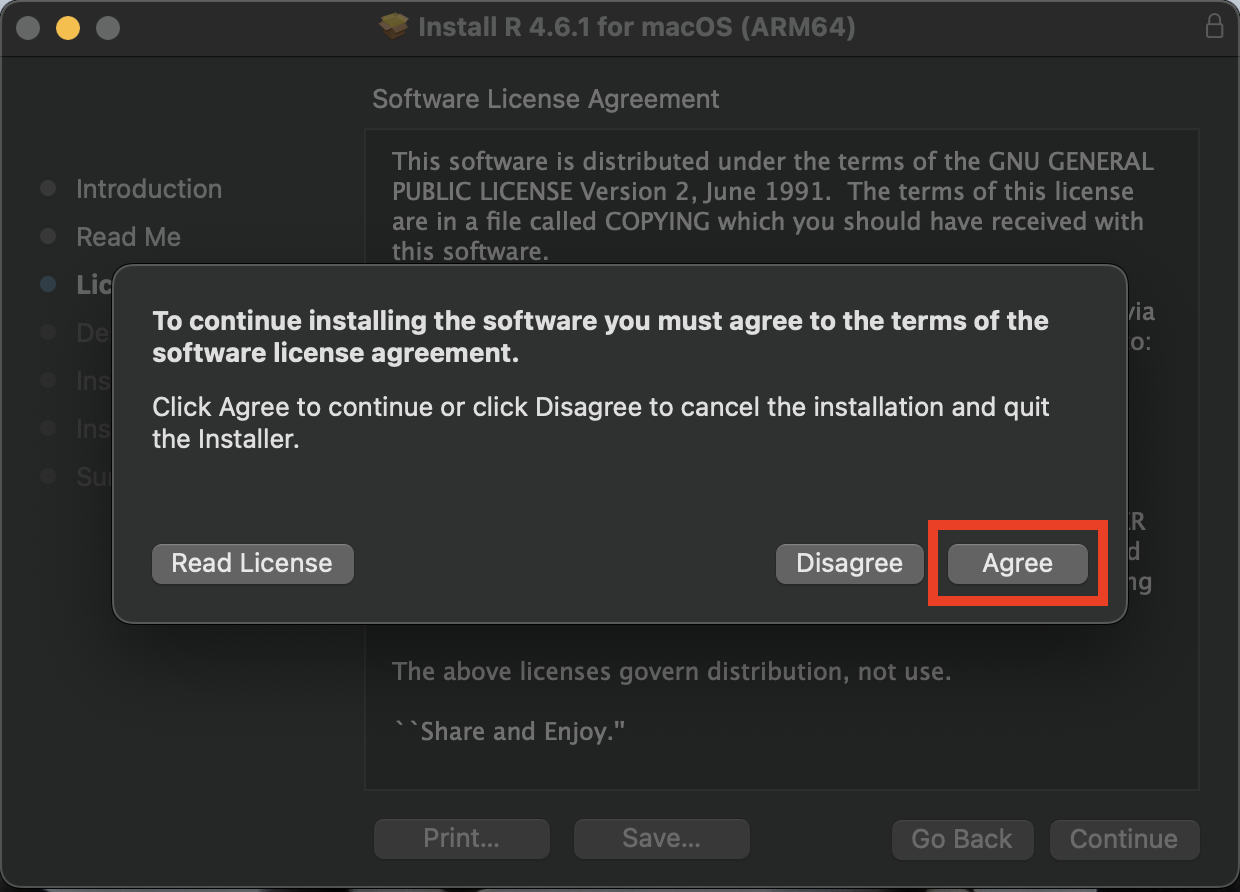
\includegraphics[width=1.1\linewidth]{R_install4.png}

  \end{columns}

\end{frame}

\begin{frame}{Download R}

  \begin{columns}[T]

    \column{0.5\textwidth}
    \centering
    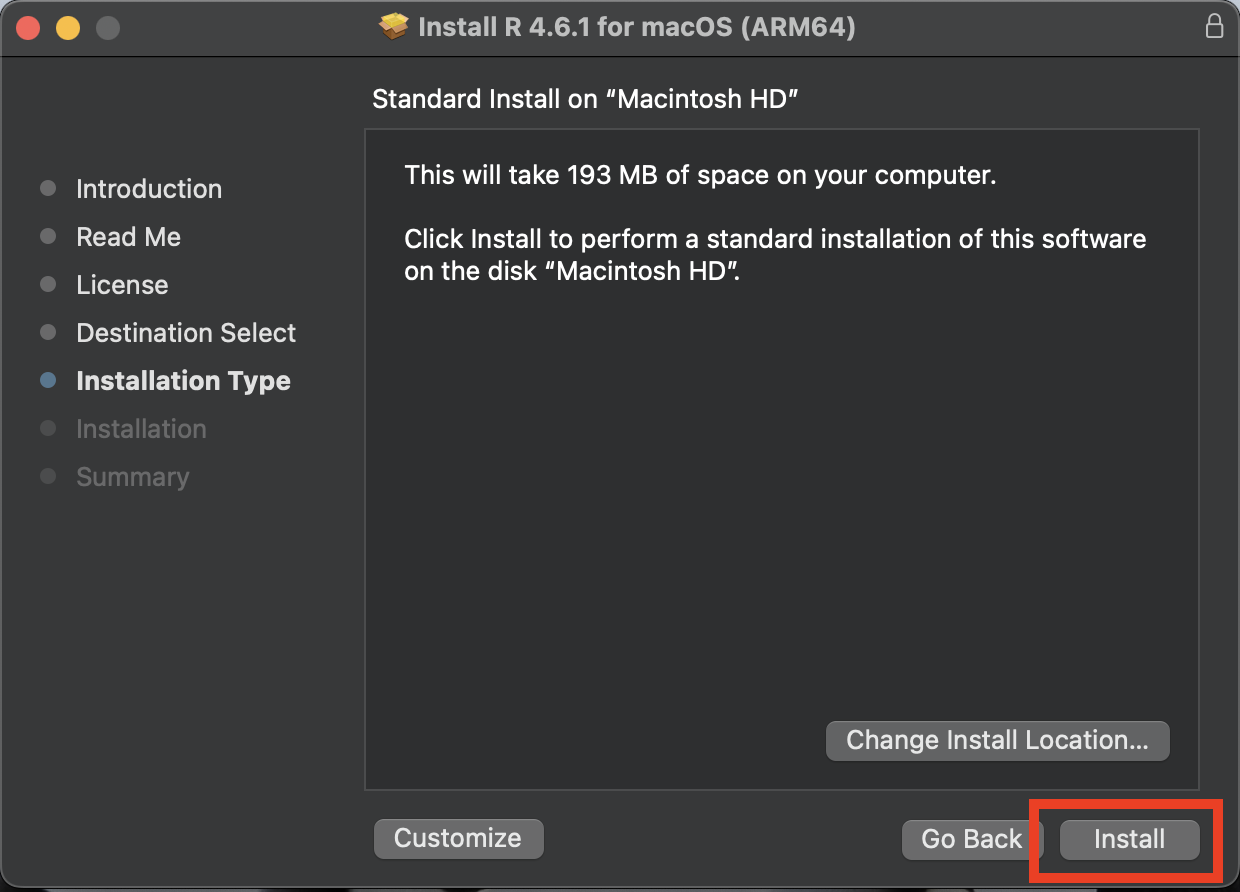
\includegraphics[width=1.1\linewidth]{R_install5.png}

    \column{0.5\textwidth}
    \centering
    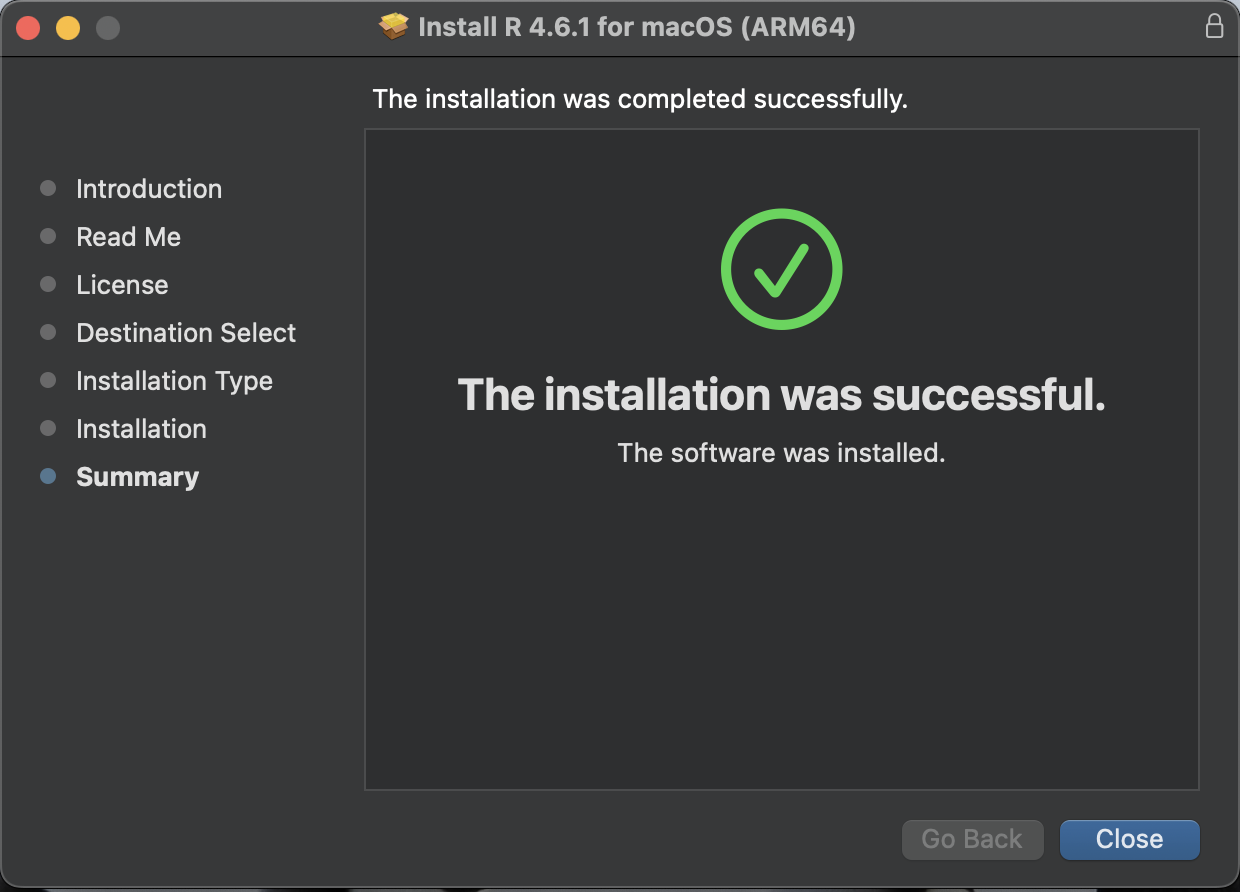
\includegraphics[width=1.1\linewidth]{R_install6.png}

  \end{columns}
\end{frame}


\begin{frame}{Download RStudio}
    \begin{figure}
        \centering
        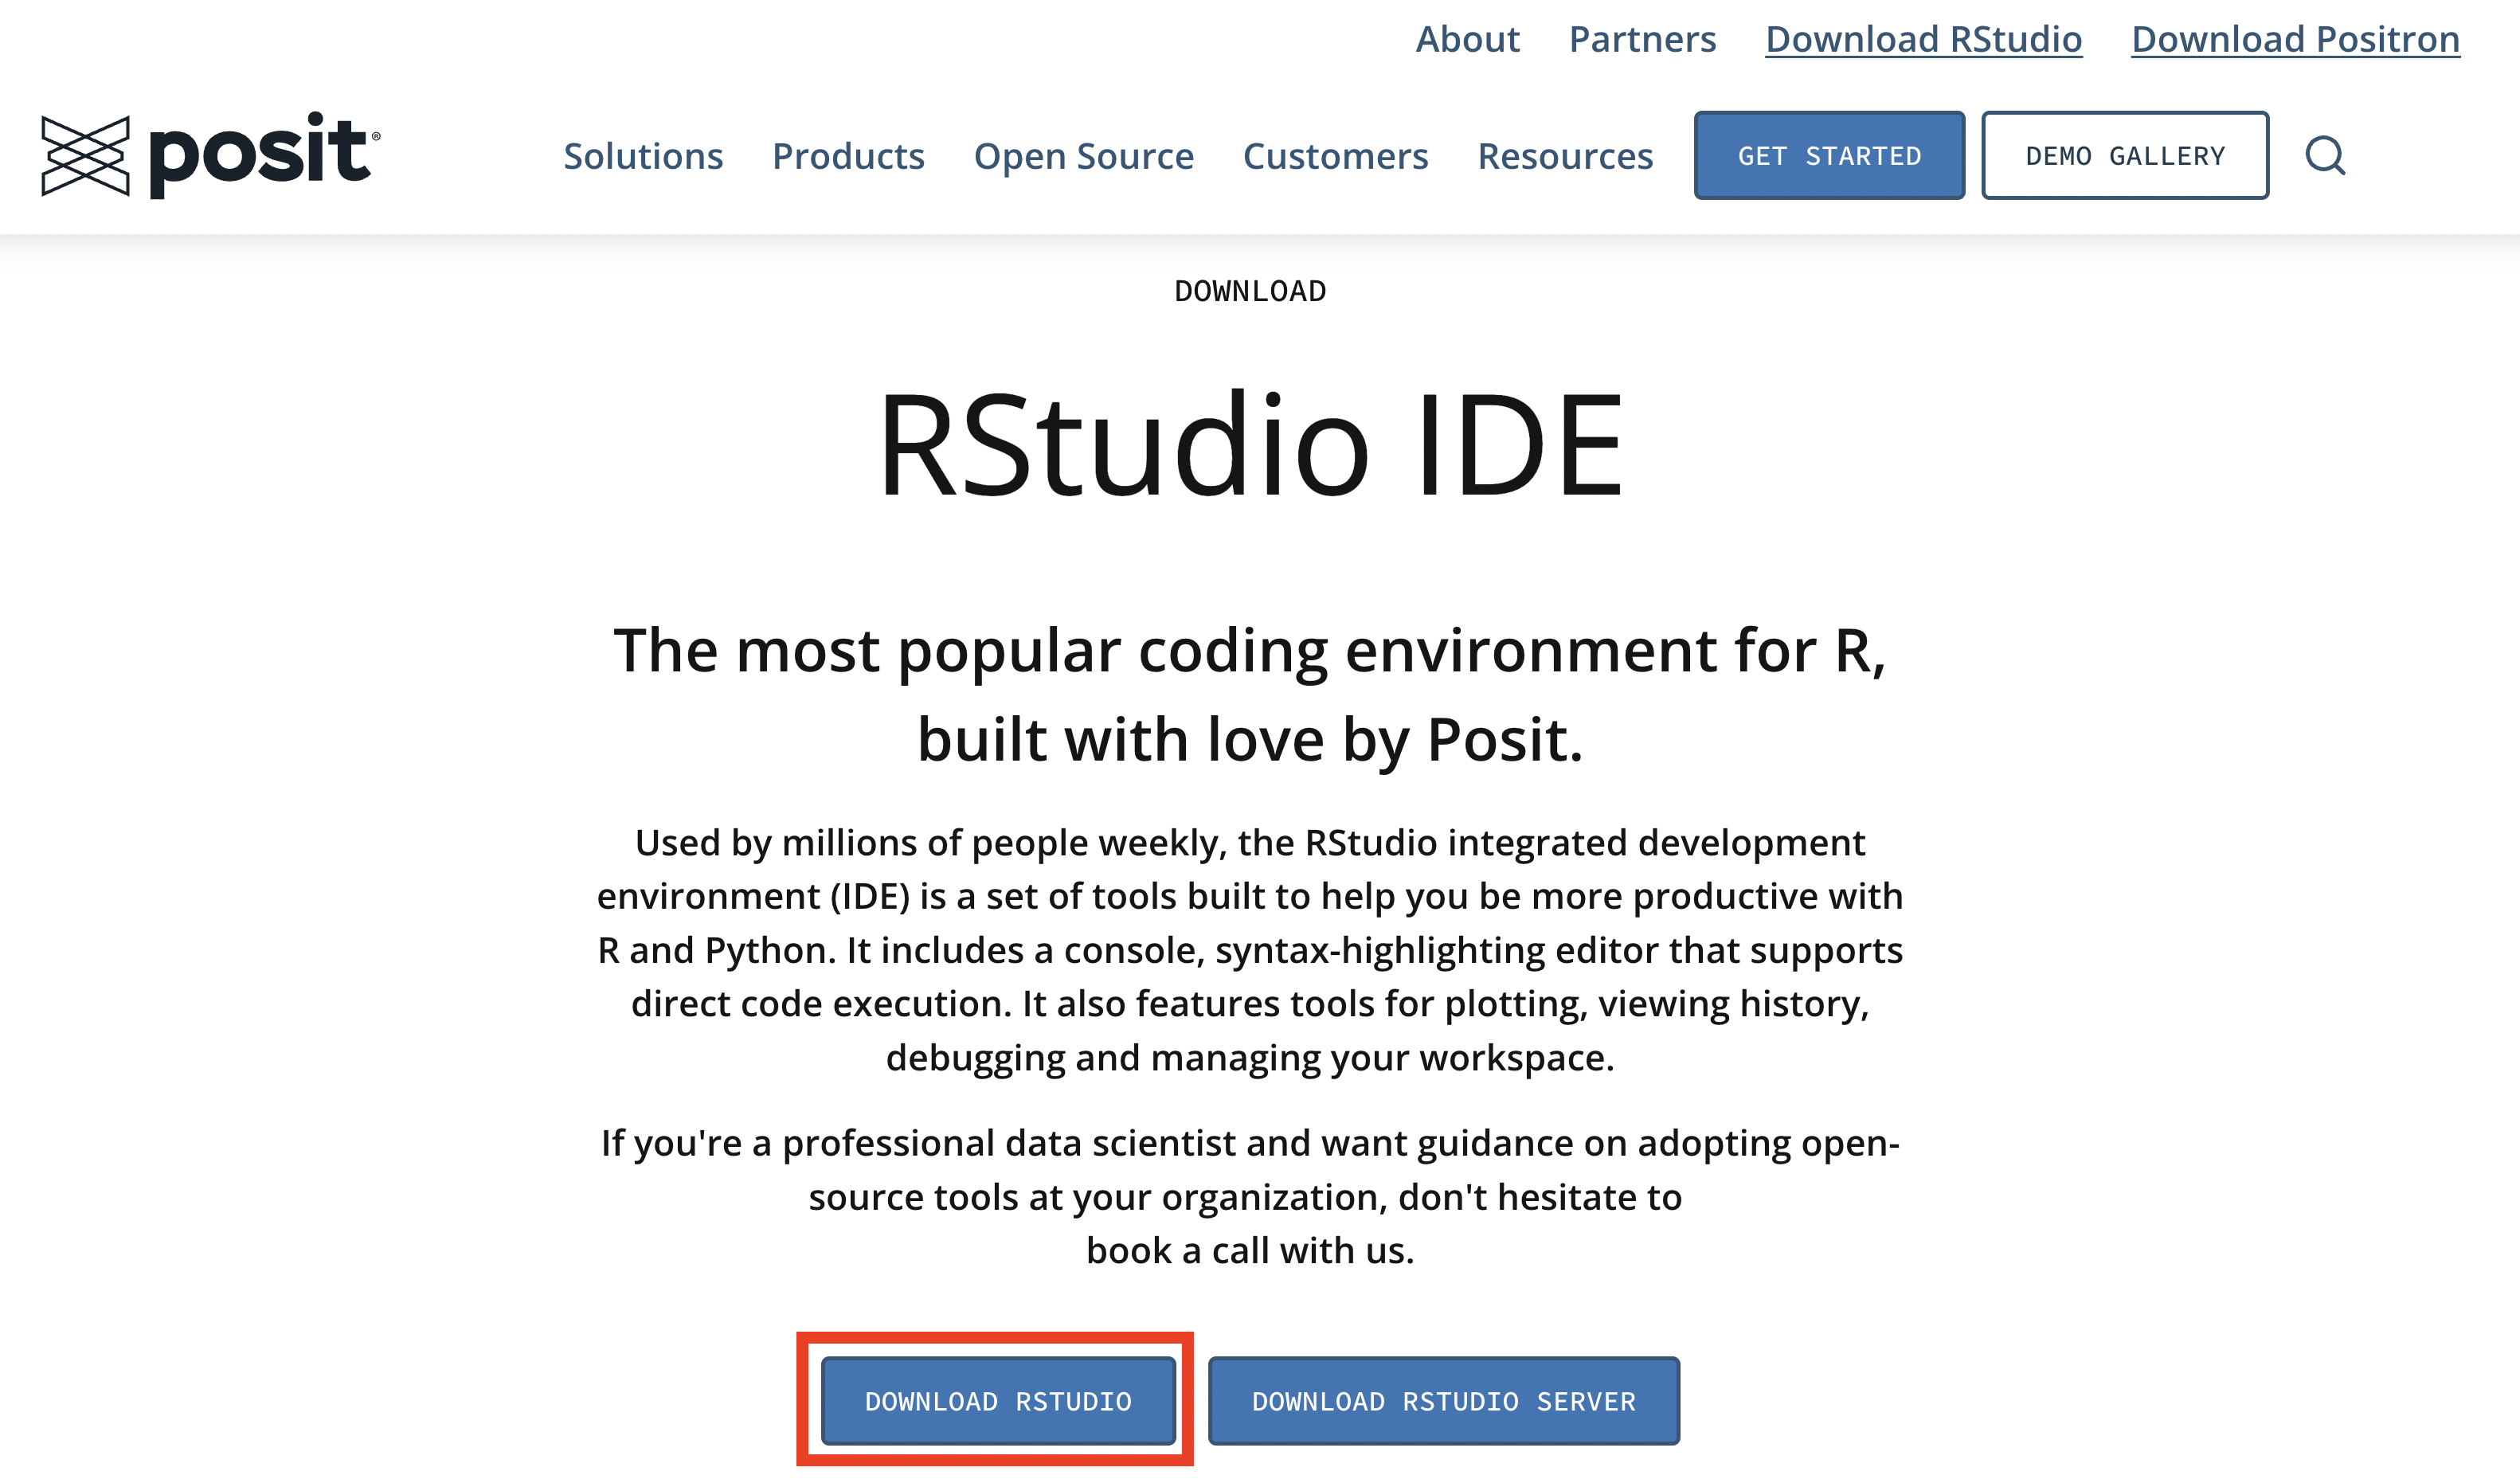
\includegraphics[width=1\linewidth]{RStudio_install1.png}
      \end{figure}
\end{frame}


\begin{frame}{Download RStudio}
    \begin{figure}
        \centering
        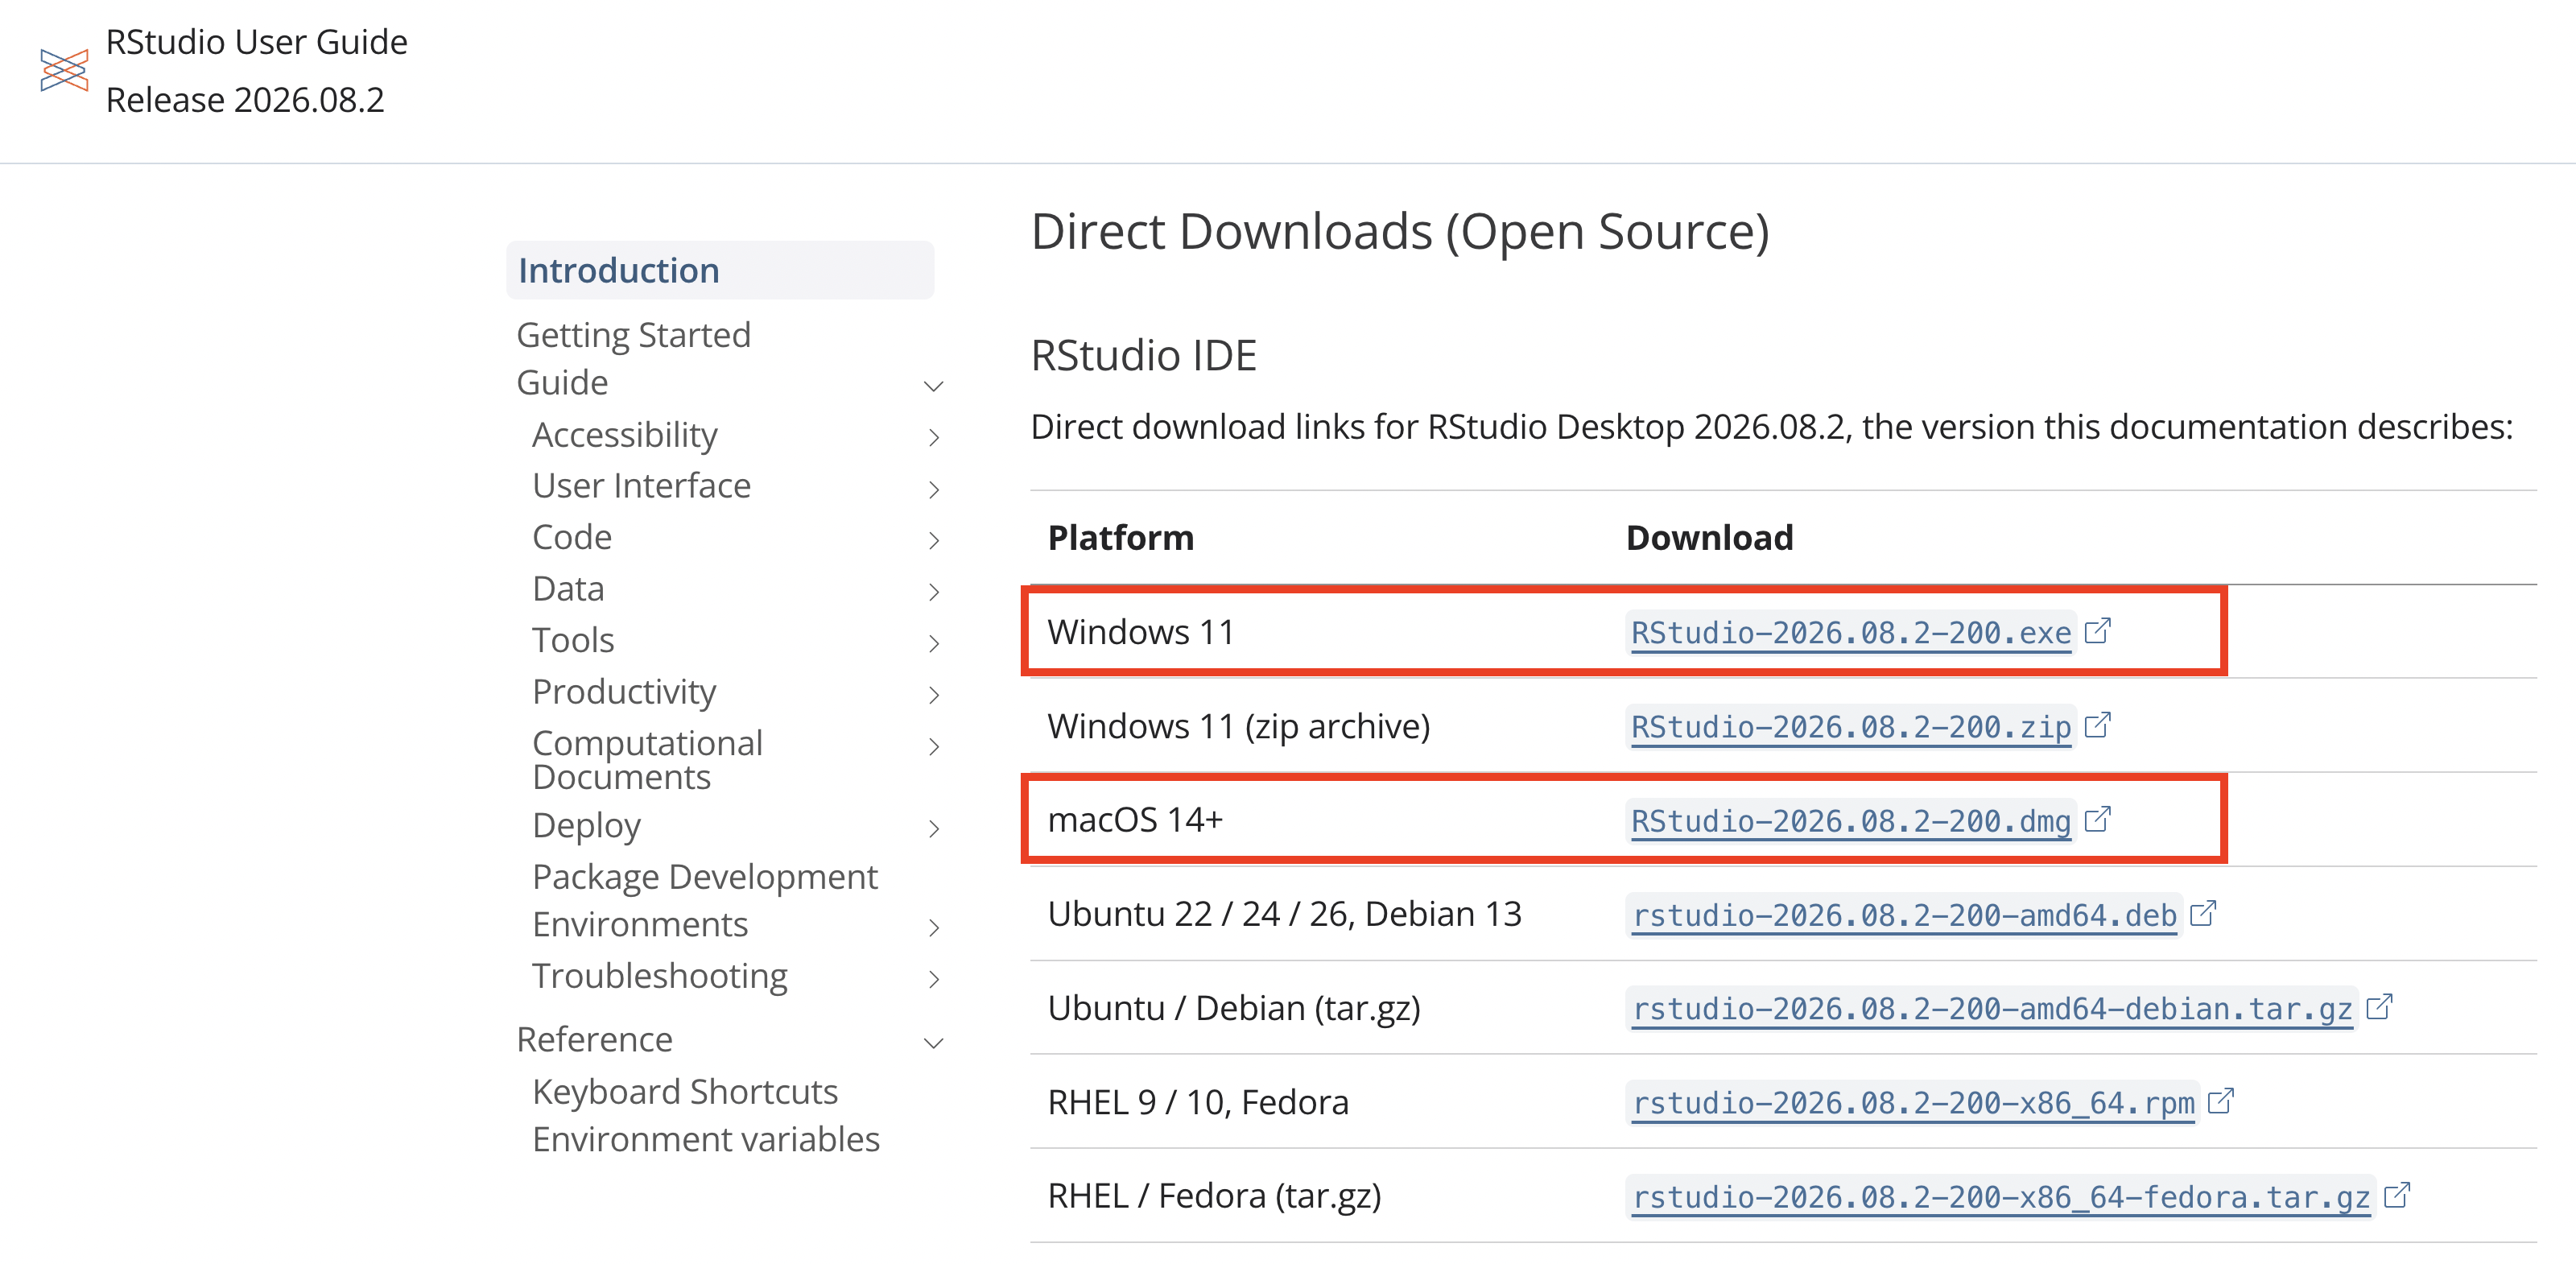
\includegraphics[width=1\linewidth]{RStudio_install2.png}
      \end{figure}
\end{frame}


\begin{frame}{Download RStudio}
  Check the application to see whether it was successfully installed
  \begin{columns}[T]

    \column{0.5\textwidth}
    \centering
    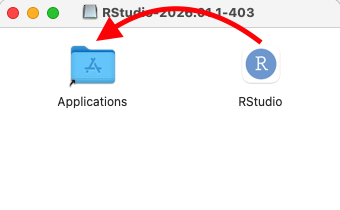
\includegraphics[width=1.1\linewidth]{截圖 2026-02-27 中午12.01.17.png}

    \column{0.5\textwidth}
    \centering
    
\includegraphics[width=1.1\linewidth]{截圖 2026-02-27 中午12.02.51.png}

  \end{columns}
\end{frame}

\begin{frame}{RStudio Interface}
  \begin{figure}
    \leftskip= -0.5cm
    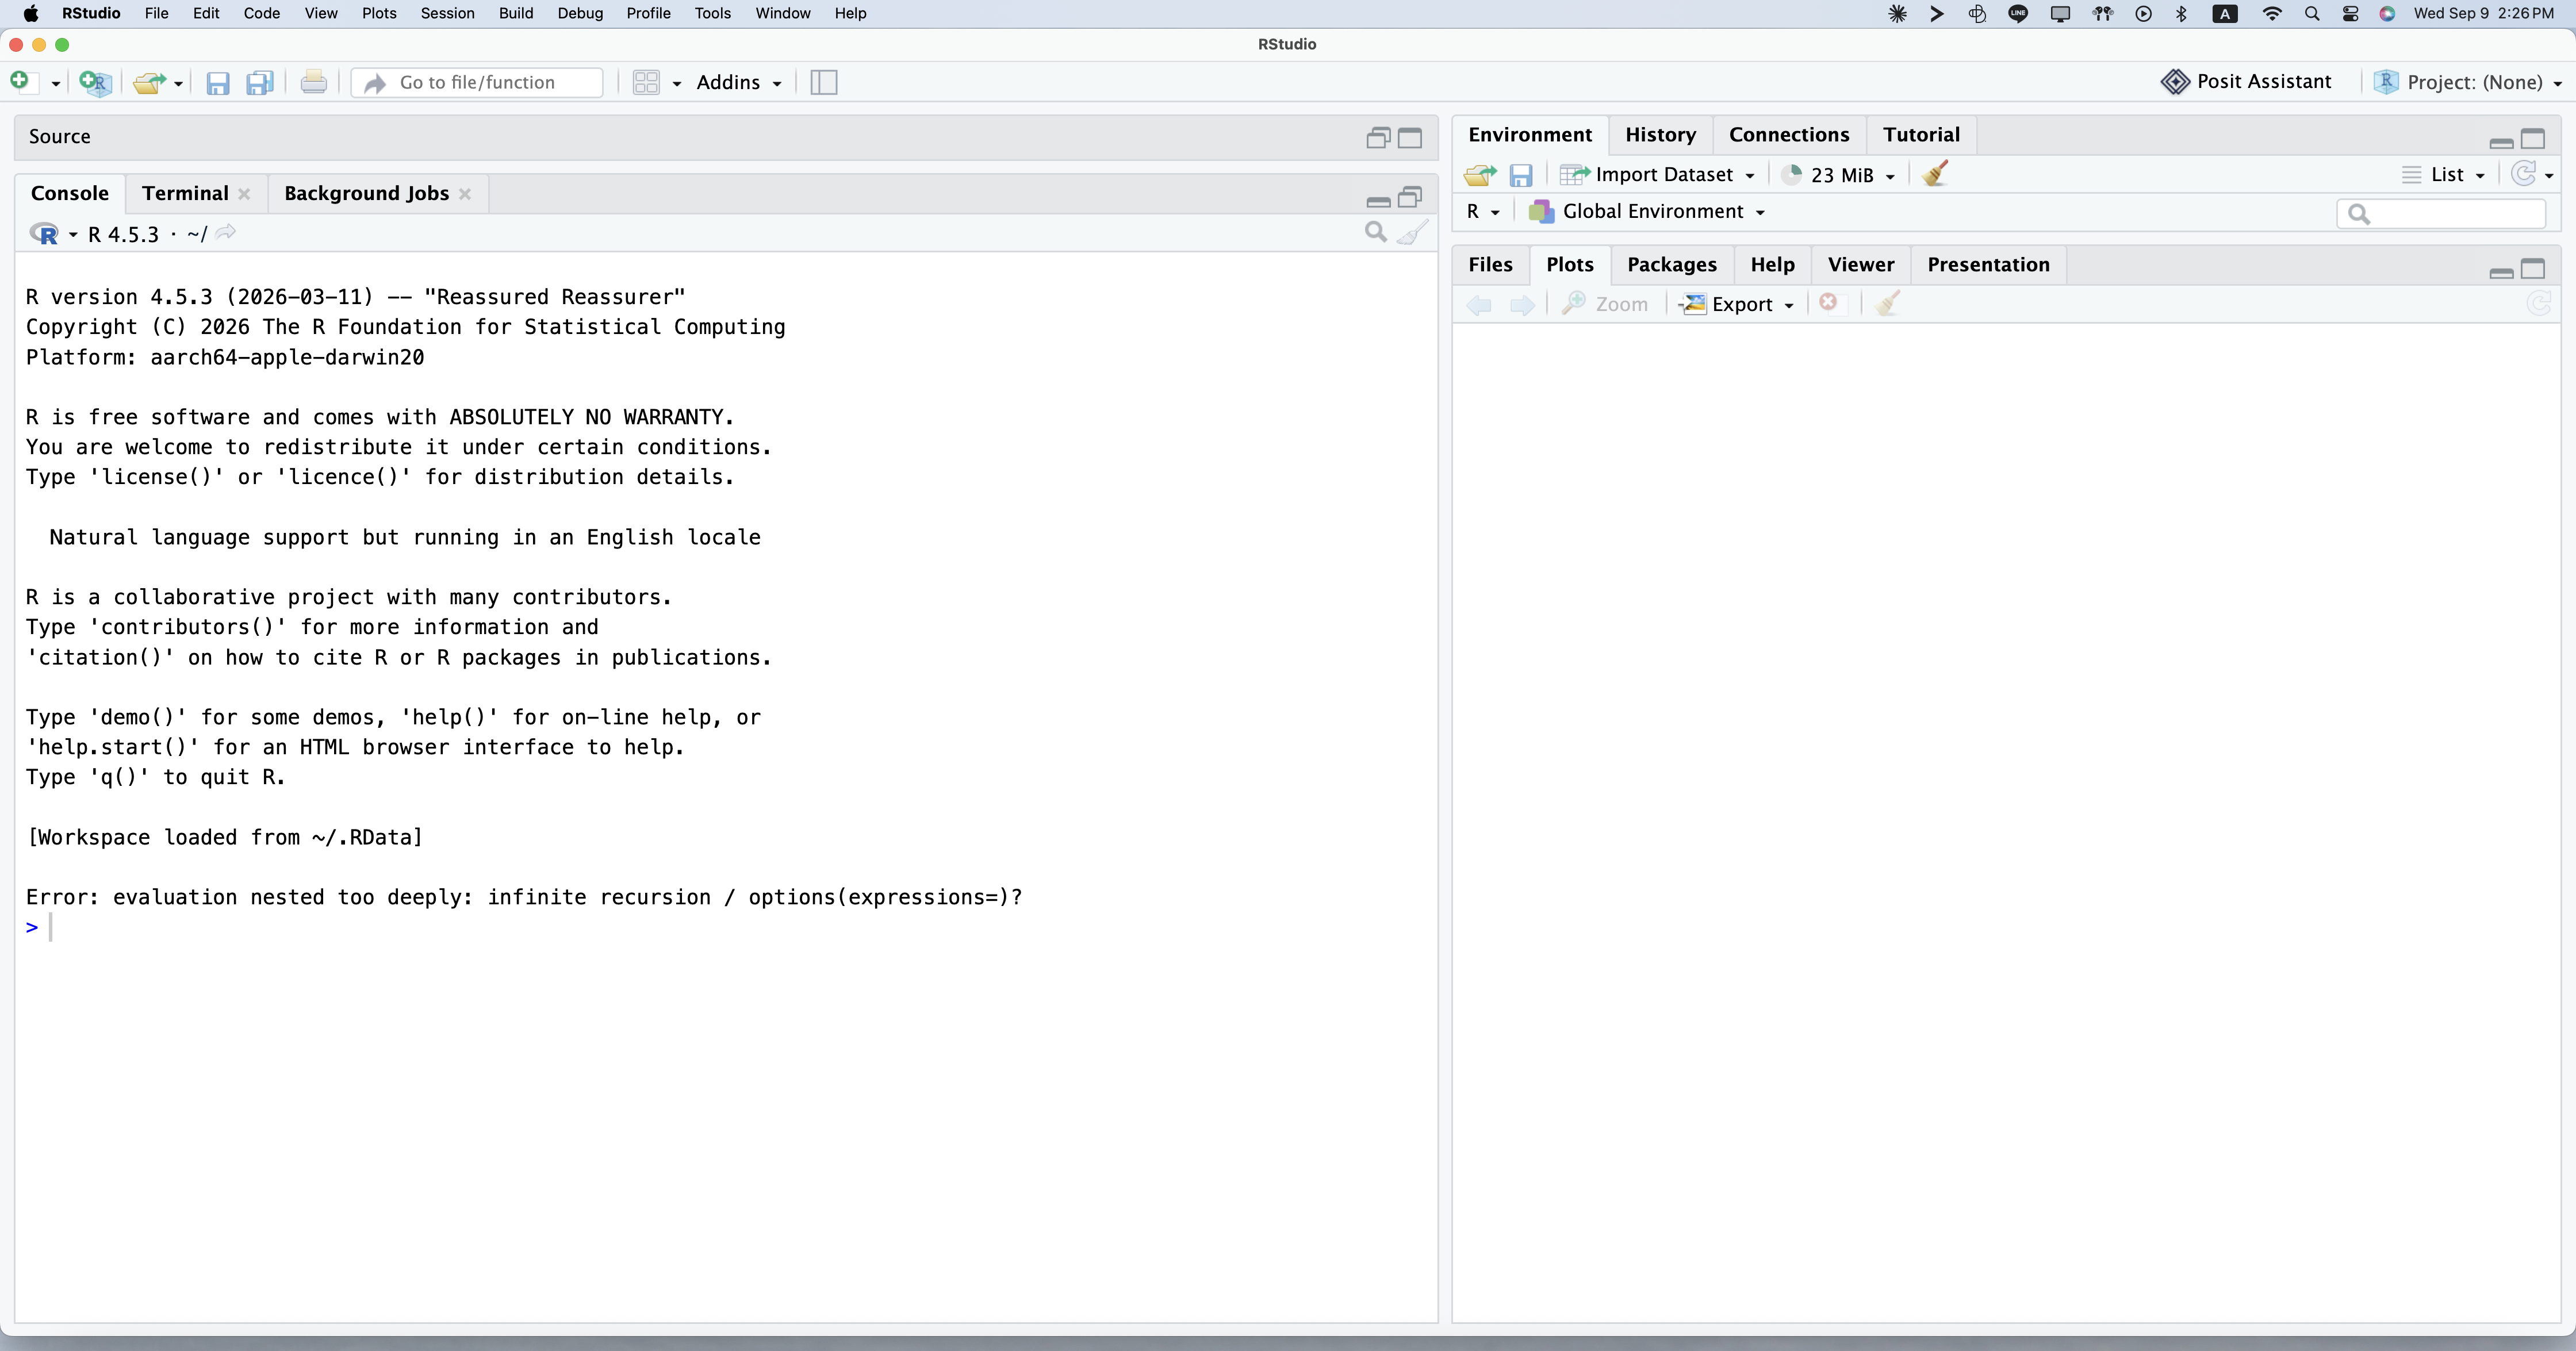
\includegraphics[width=1.1\linewidth]{R_overview.png}
  \end{figure}
\end{frame}

\begin{frame}{Change the Appearance}
  Tools $\rightarrow$ Global Option $\rightarrow$ Appearance
  \begin{columns}[T]

    \column{0.5\textwidth}
    \centering
    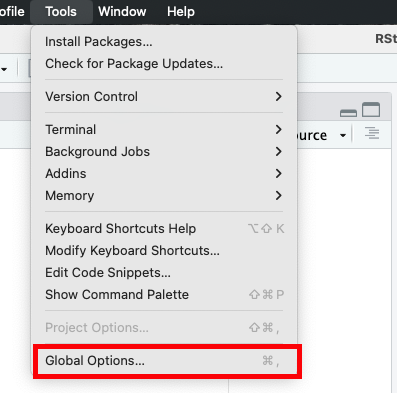
\includegraphics[width=1.1\linewidth]{截圖 2026-02-27 下午3.47.31.png}

    \column{0.5\textwidth}
    \centering
    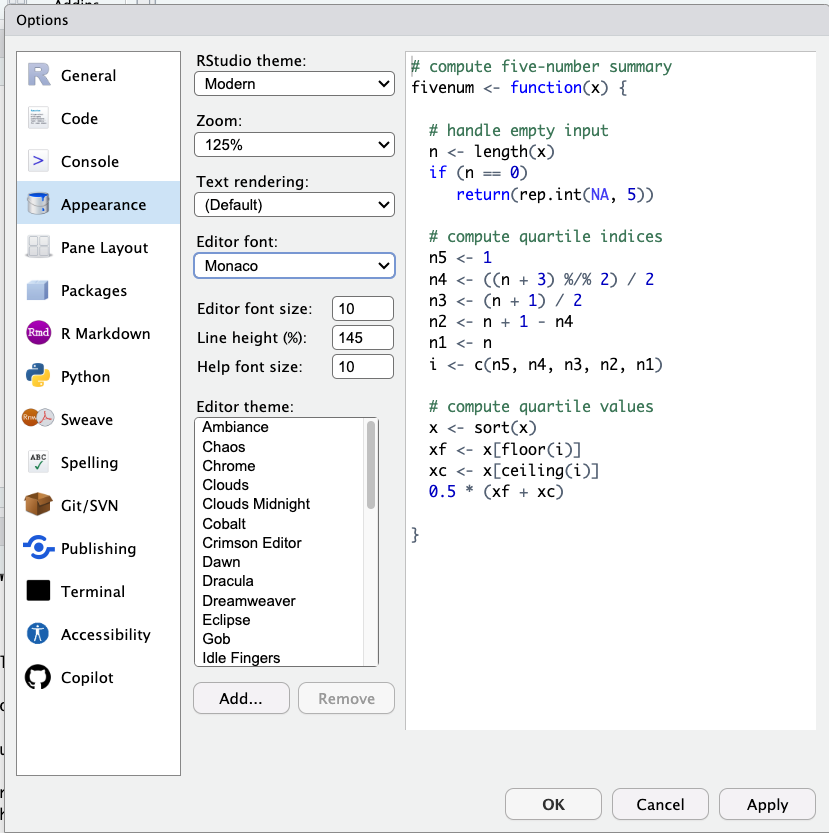
\includegraphics[width=1.1\linewidth]{截圖 2026-02-27 下午3.47.00.png}

  \end{columns}
\end{frame}

\begin{frame}{RStudio Interface}
  \begin{itemize}
    \item Command: The code you type into the console
    \item Commnad Line: The area where you type commands.
  \end{itemize}
  \begin{figure}
    \leftskip= -0.5cm
    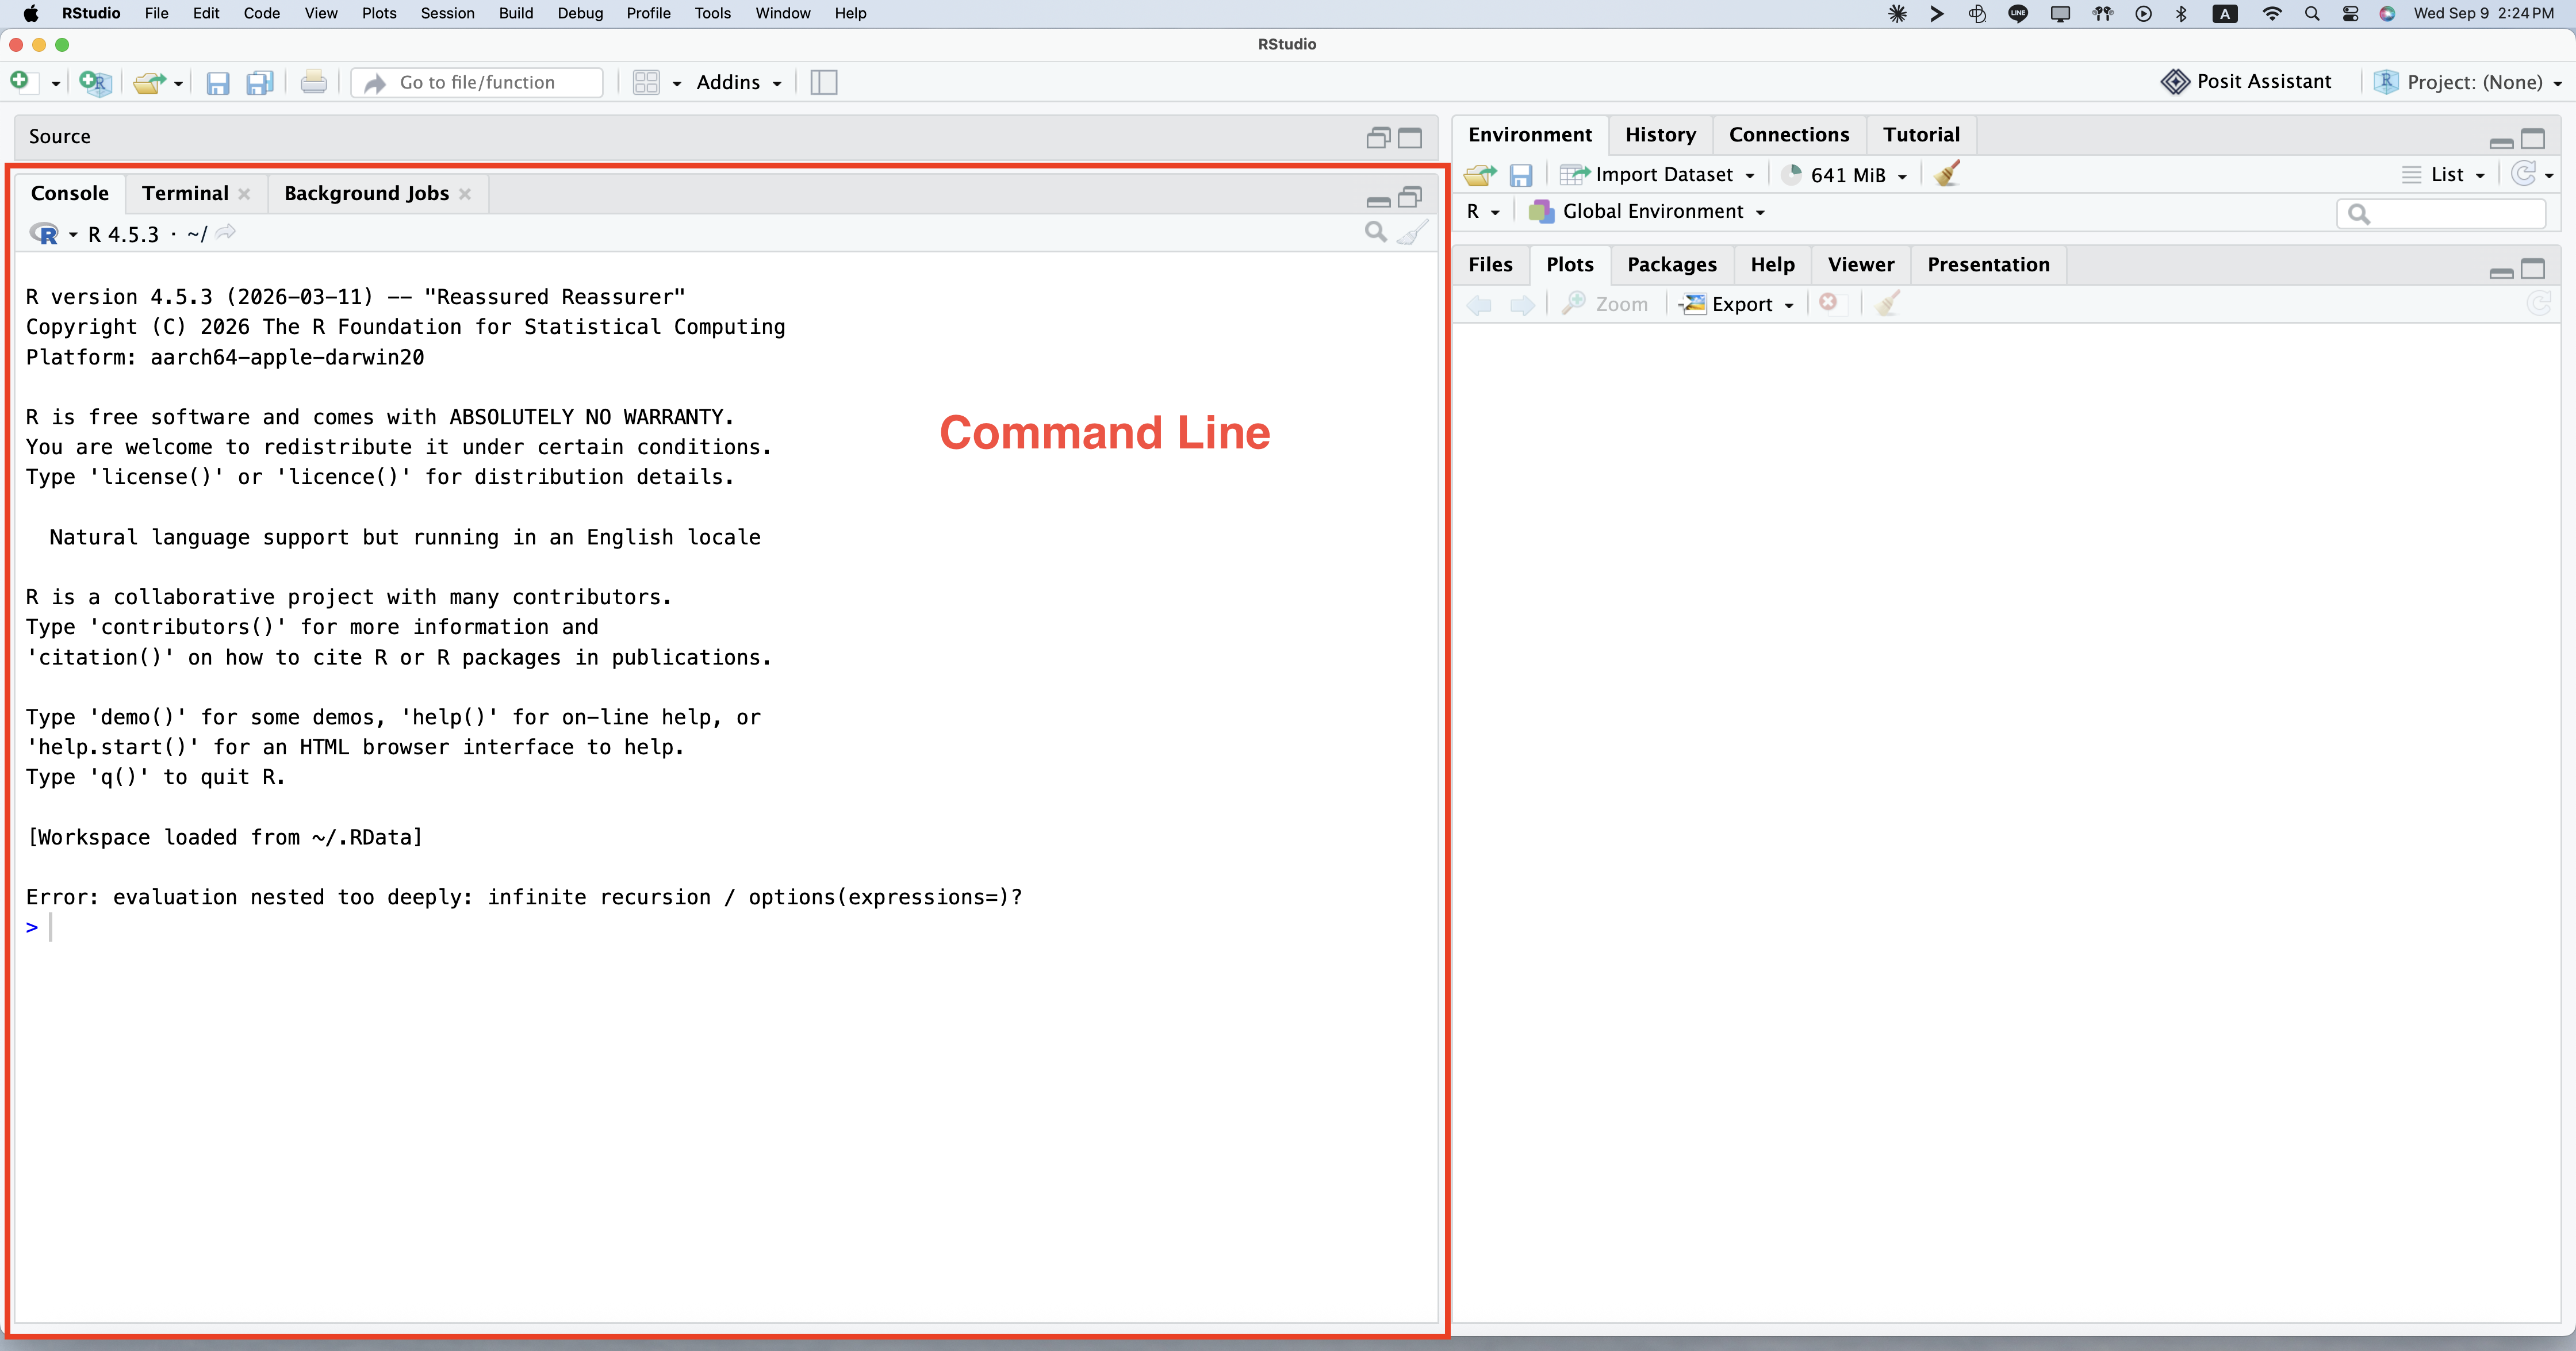
\includegraphics[width=1.1\linewidth]{R_command_pane.png}
  \end{figure}
\end{frame}


\begin{frame}[fragile]{Some Simple Commands}
  Here are some simple command you can play around with
  \begin{itemize}
    \item Arithmetic operator: $+$, $-$, $*$, $/$, \verb|^|, \verb|%/%|, \verb|%%|
    \item The colon operator (:) creates a sequence of numbers.
    \item Hash symbol (\#) is used to add comments in R code.
  \end{itemize}
  \begin{figure}
    \leftskip= -0.5cm
    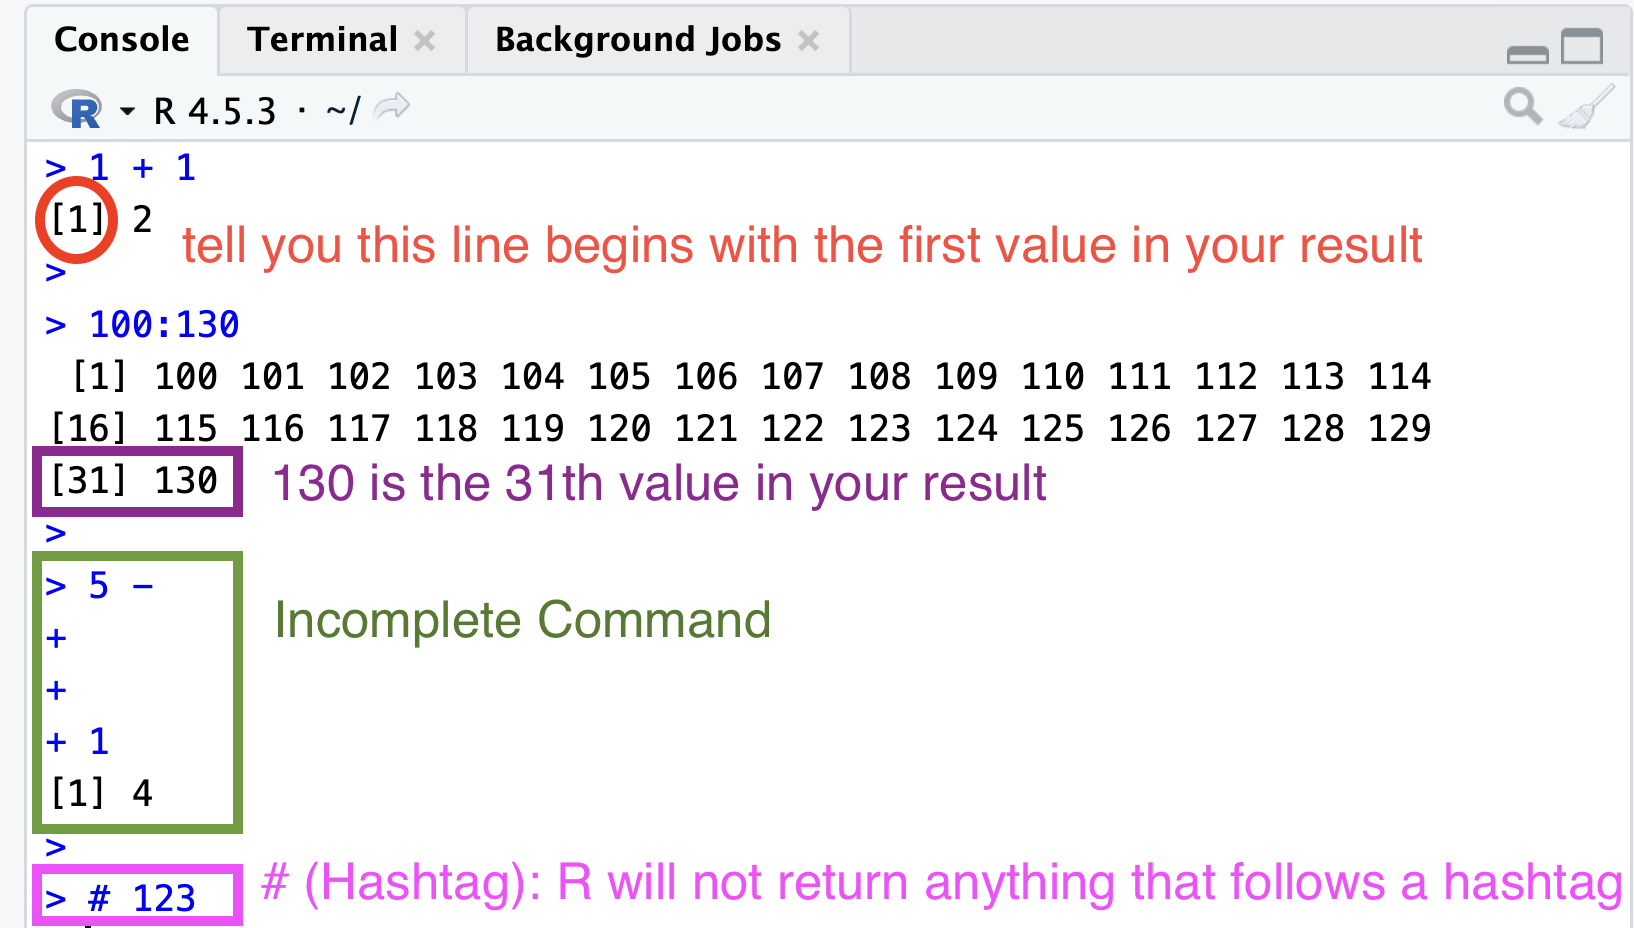
\includegraphics[width=1\linewidth]{R_console_demo.png}
  \end{figure}
\end{frame}


\begin{frame}{Basic Arithmetic Operations}
  \begin{columns}[T]

    \column{0.6\textwidth}
    The basic arithmetic operators are:
    \begin{itemize}
      \item + (addition)
      \item - (subtraction)
      \item * (multiplication)
      \item / (division)
      \item \texttt{\^} (exponentiation)
      \item \%/\% (quotient)
      \item \%\% (modulus)
    \end{itemize}

    \column{0.5\textwidth}
    \centering
    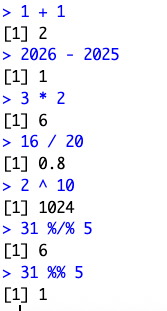
\includegraphics[width=0.65\linewidth]{截圖 2026-02-27 下午4.06.52.png}

  \end{columns}
\end{frame}

\begin{frame}{Basic Arithmetic Function}
  \begin{columns}
    \column{0.6\textwidth}

    \textbf{Functions} accept \textbf{parameters} (in
    parentheses) and return a value. \\
    \vspace{15 pt}
    The basic arithmetic functions are:
    \begin{itemize}
      \item log(x): logarithms base e of x
      \item exp(x): exponential of x
      \item abs(x): absolute value of x
      \item sqrt(x): square root of x
    \end{itemize}

    \column{0.45\textwidth}
    \begin{figure}
      \centering
      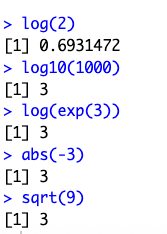
\includegraphics[width=0.9\linewidth]{截圖 2026-02-27 下午4.23.55.png}
    \end{figure}
  \end{columns}

\end{frame}

\begin{frame}{Objects}
  \begin{columns}
    \column{0.75\textwidth}
    \begin{itemize}
      \item Objects are named containers for data.
      \item The assignment operator in R is: \texttt{<-} or \texttt{=}
      \item Variable names can start with a letter
      \begin{itemize}
        \item Just not a number by itself.
        \item Examples: result, x1
      \end{itemize}
      \item R is case sensitive (i.e. Result $\neq$ result)
      \item Use \texttt{rm()} to remove objects from the environment.
    \end{itemize}

    \column{0.45\textwidth}
    \begin{figure}
      \centering
      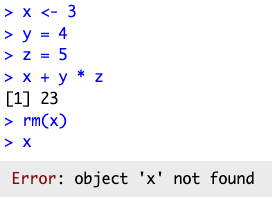
\includegraphics[width=1\linewidth]{截圖 2026-02-27 下午4.55.17.png}
    \end{figure}
  \end{columns}
\end{frame}

\begin{frame}{Environment Pane}
    \begin{itemize}
    \item The Environment tab shows all the objects you have created.
    \item You can click on an object to view its contents.
    \item You can also use the Environment tab to remove objects.
    \end{itemize}
    
    \begin{figure}
        \centering
        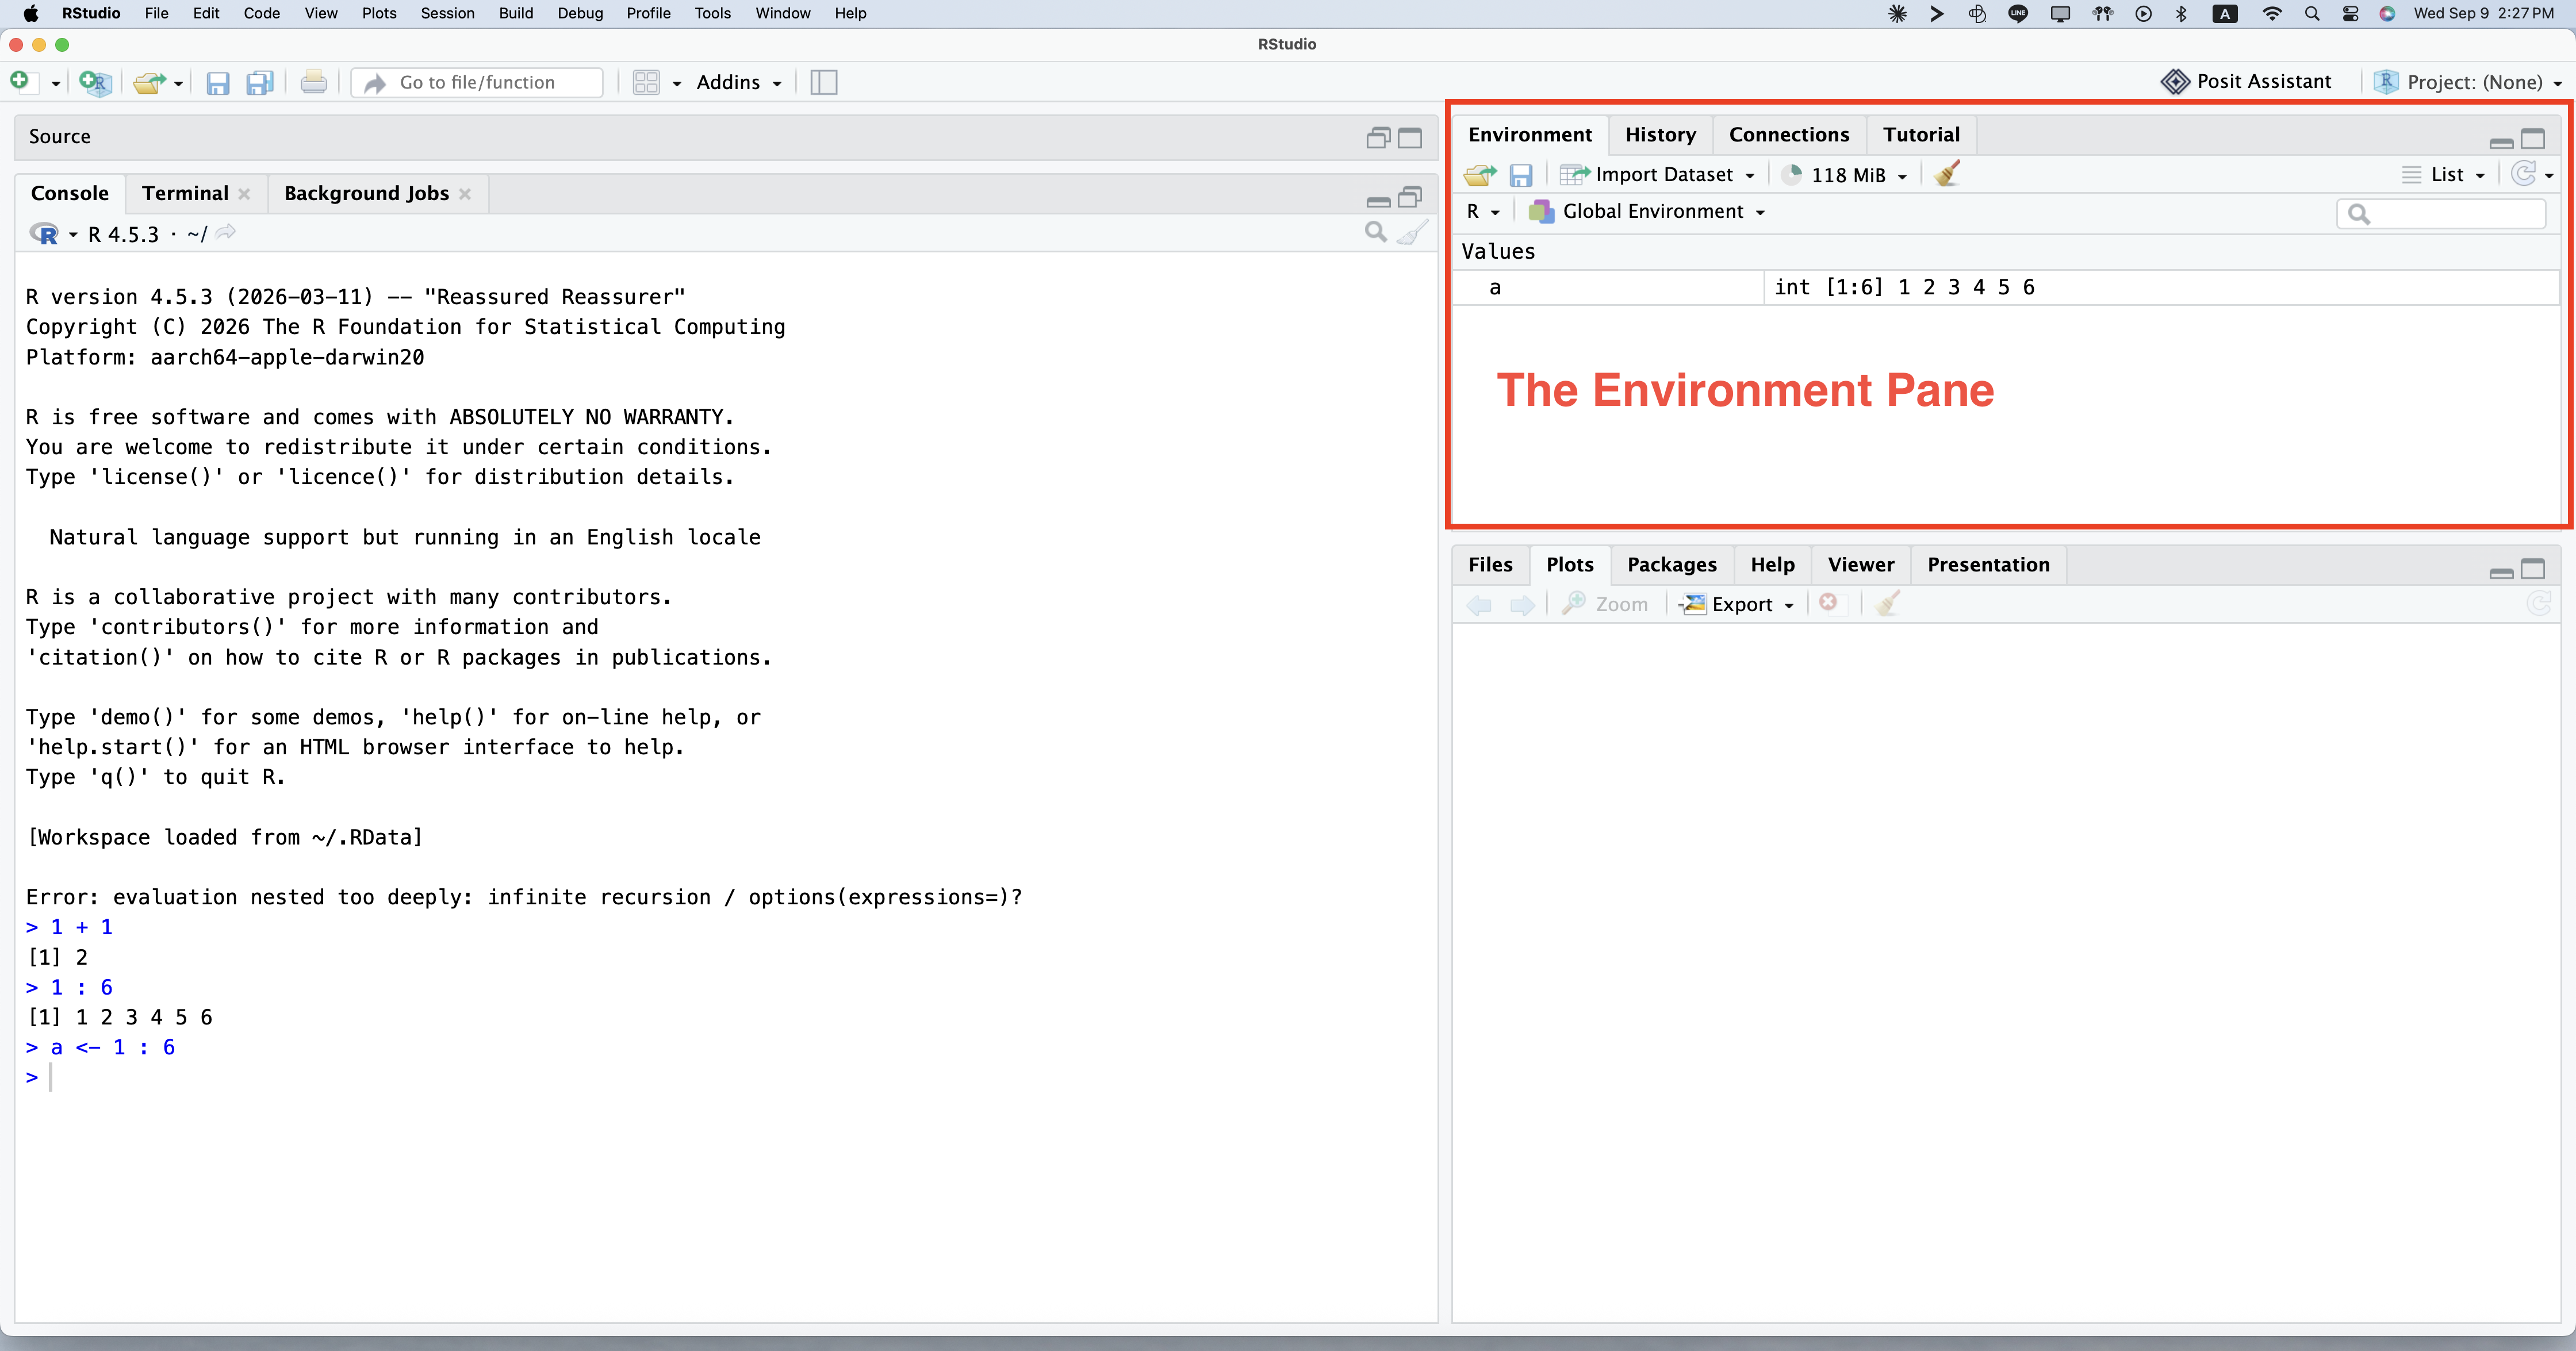
\includegraphics[width=1\linewidth]{R_environment_pane.png}
    \end{figure}
\end{frame}


\begin{frame}{Script}
    What you type in the command line cannot be saved \\
    What should you do if you want to save your code? \\
    \vspace{10pt}
    \large{R script}
    \begin{itemize}
        \item A text file containing a sequence of R commands
        \item You can save your code in a script and run it later
    \end{itemize}
    \begin{figure}
        \centering
        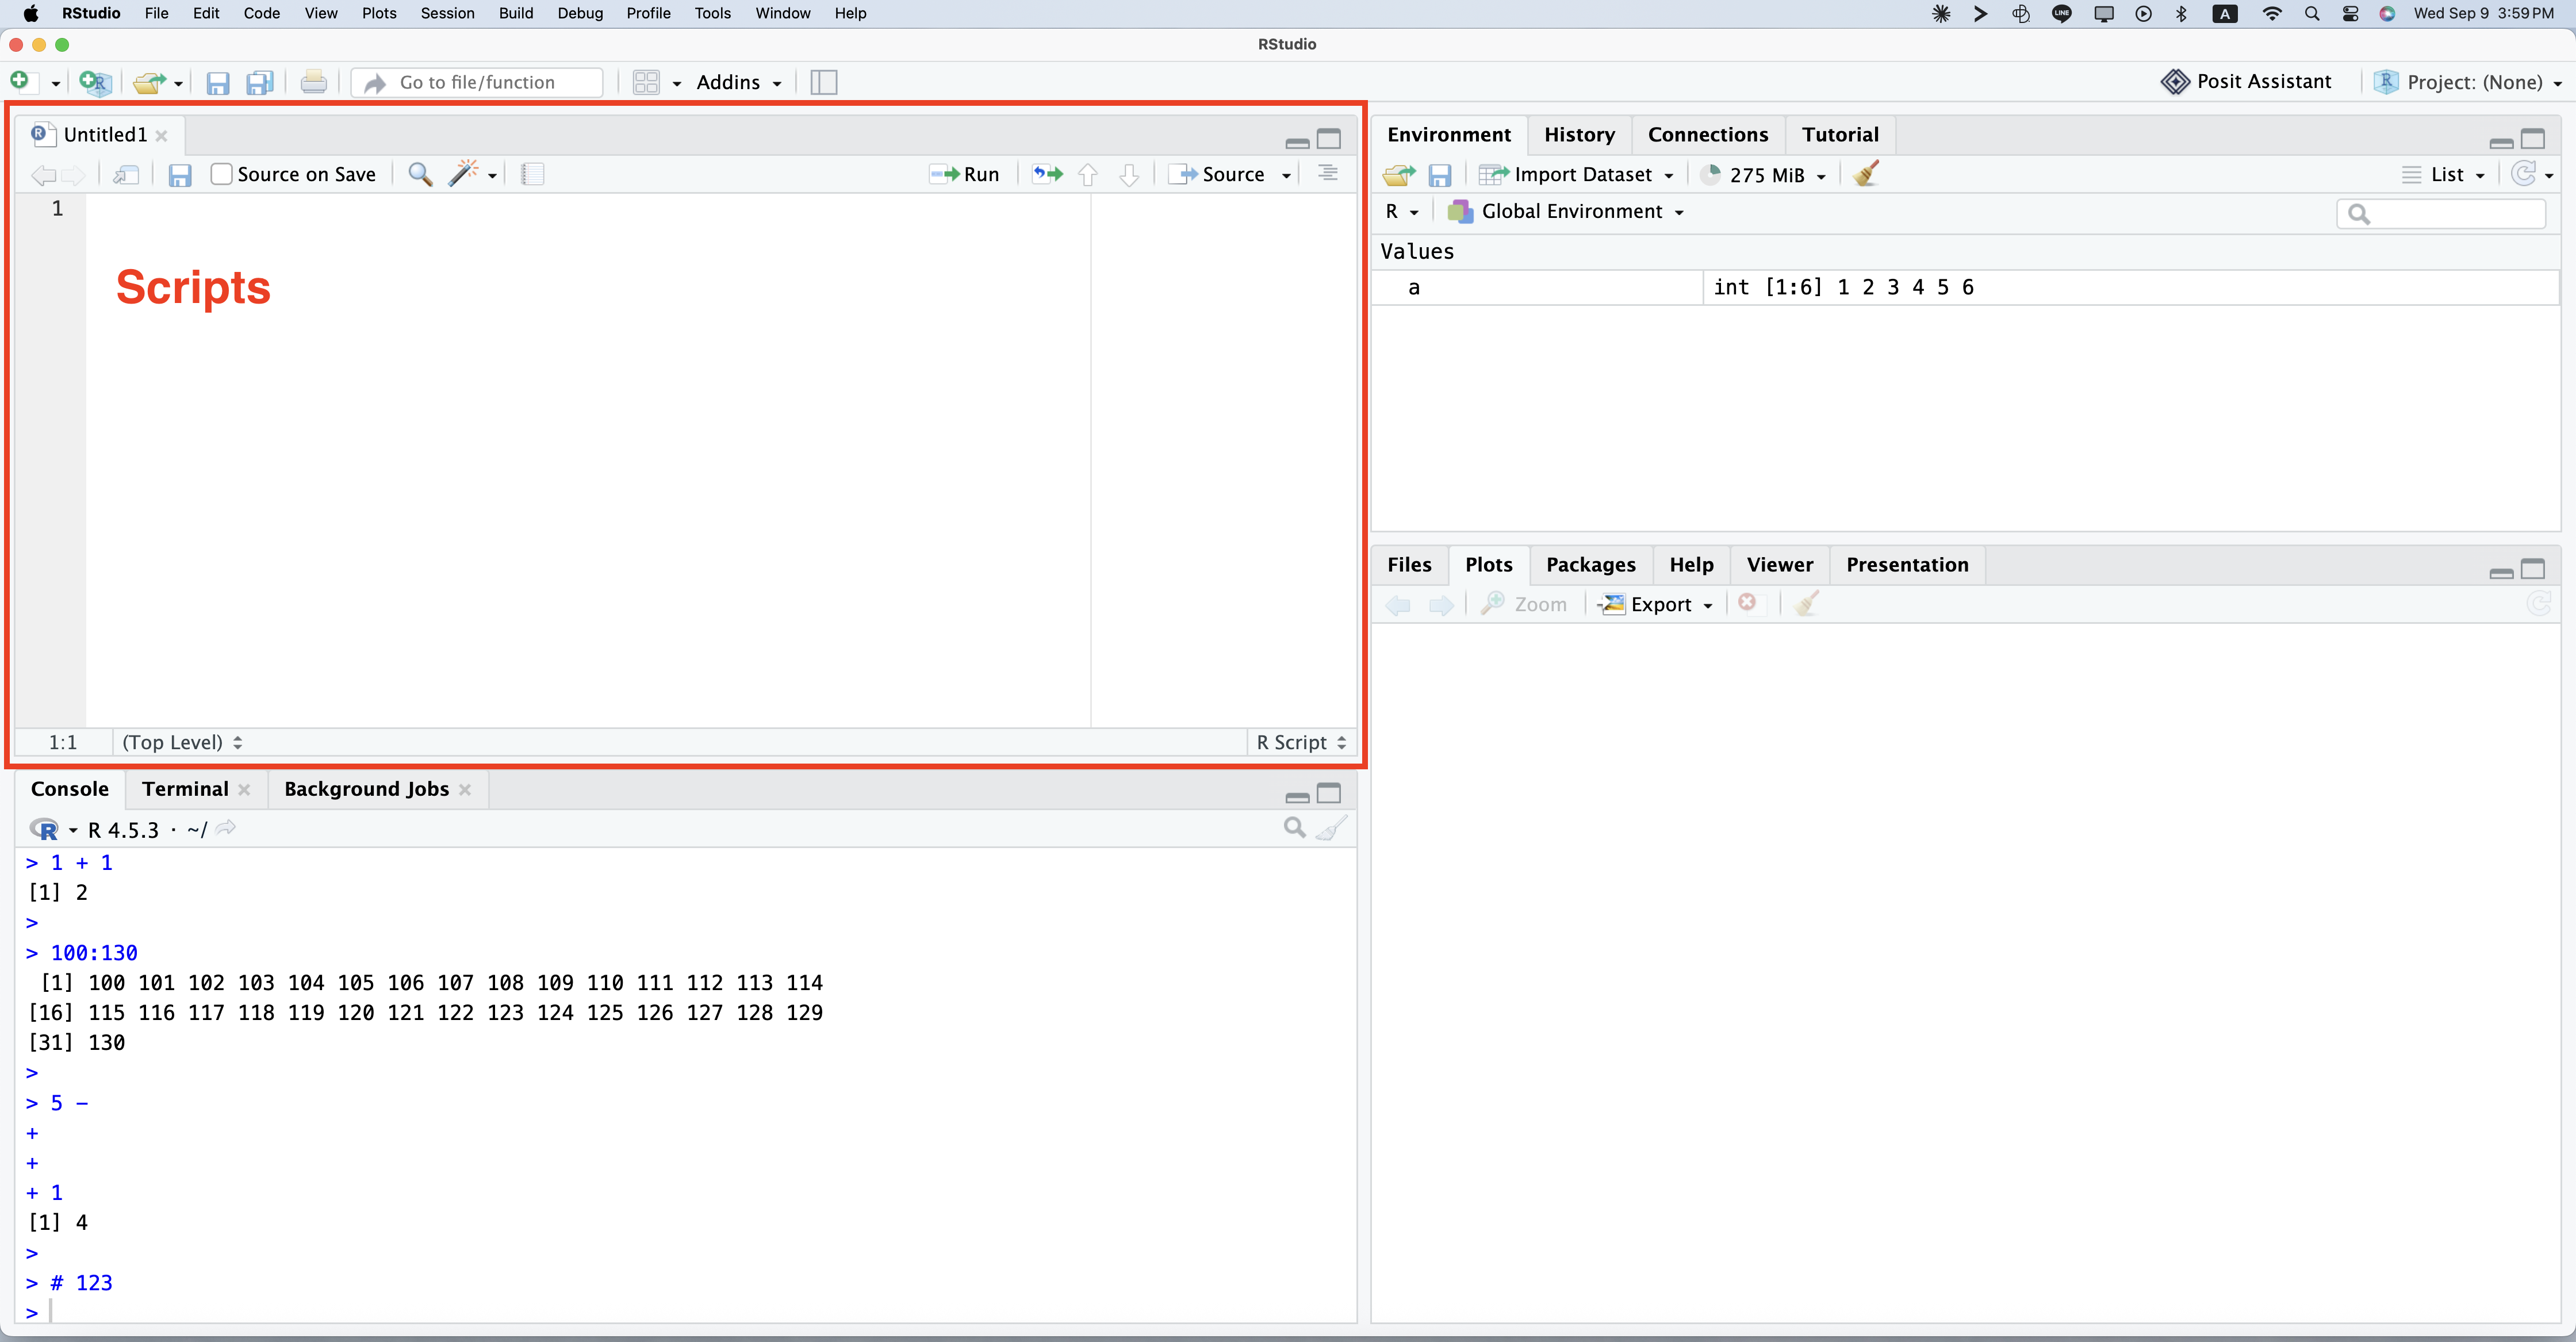
\includegraphics[width=1\linewidth]{R_script1.png}
    \end{figure}

\end{frame}

\begin{frame}{How to run code in the script}
    \begin{figure}
        \centering
        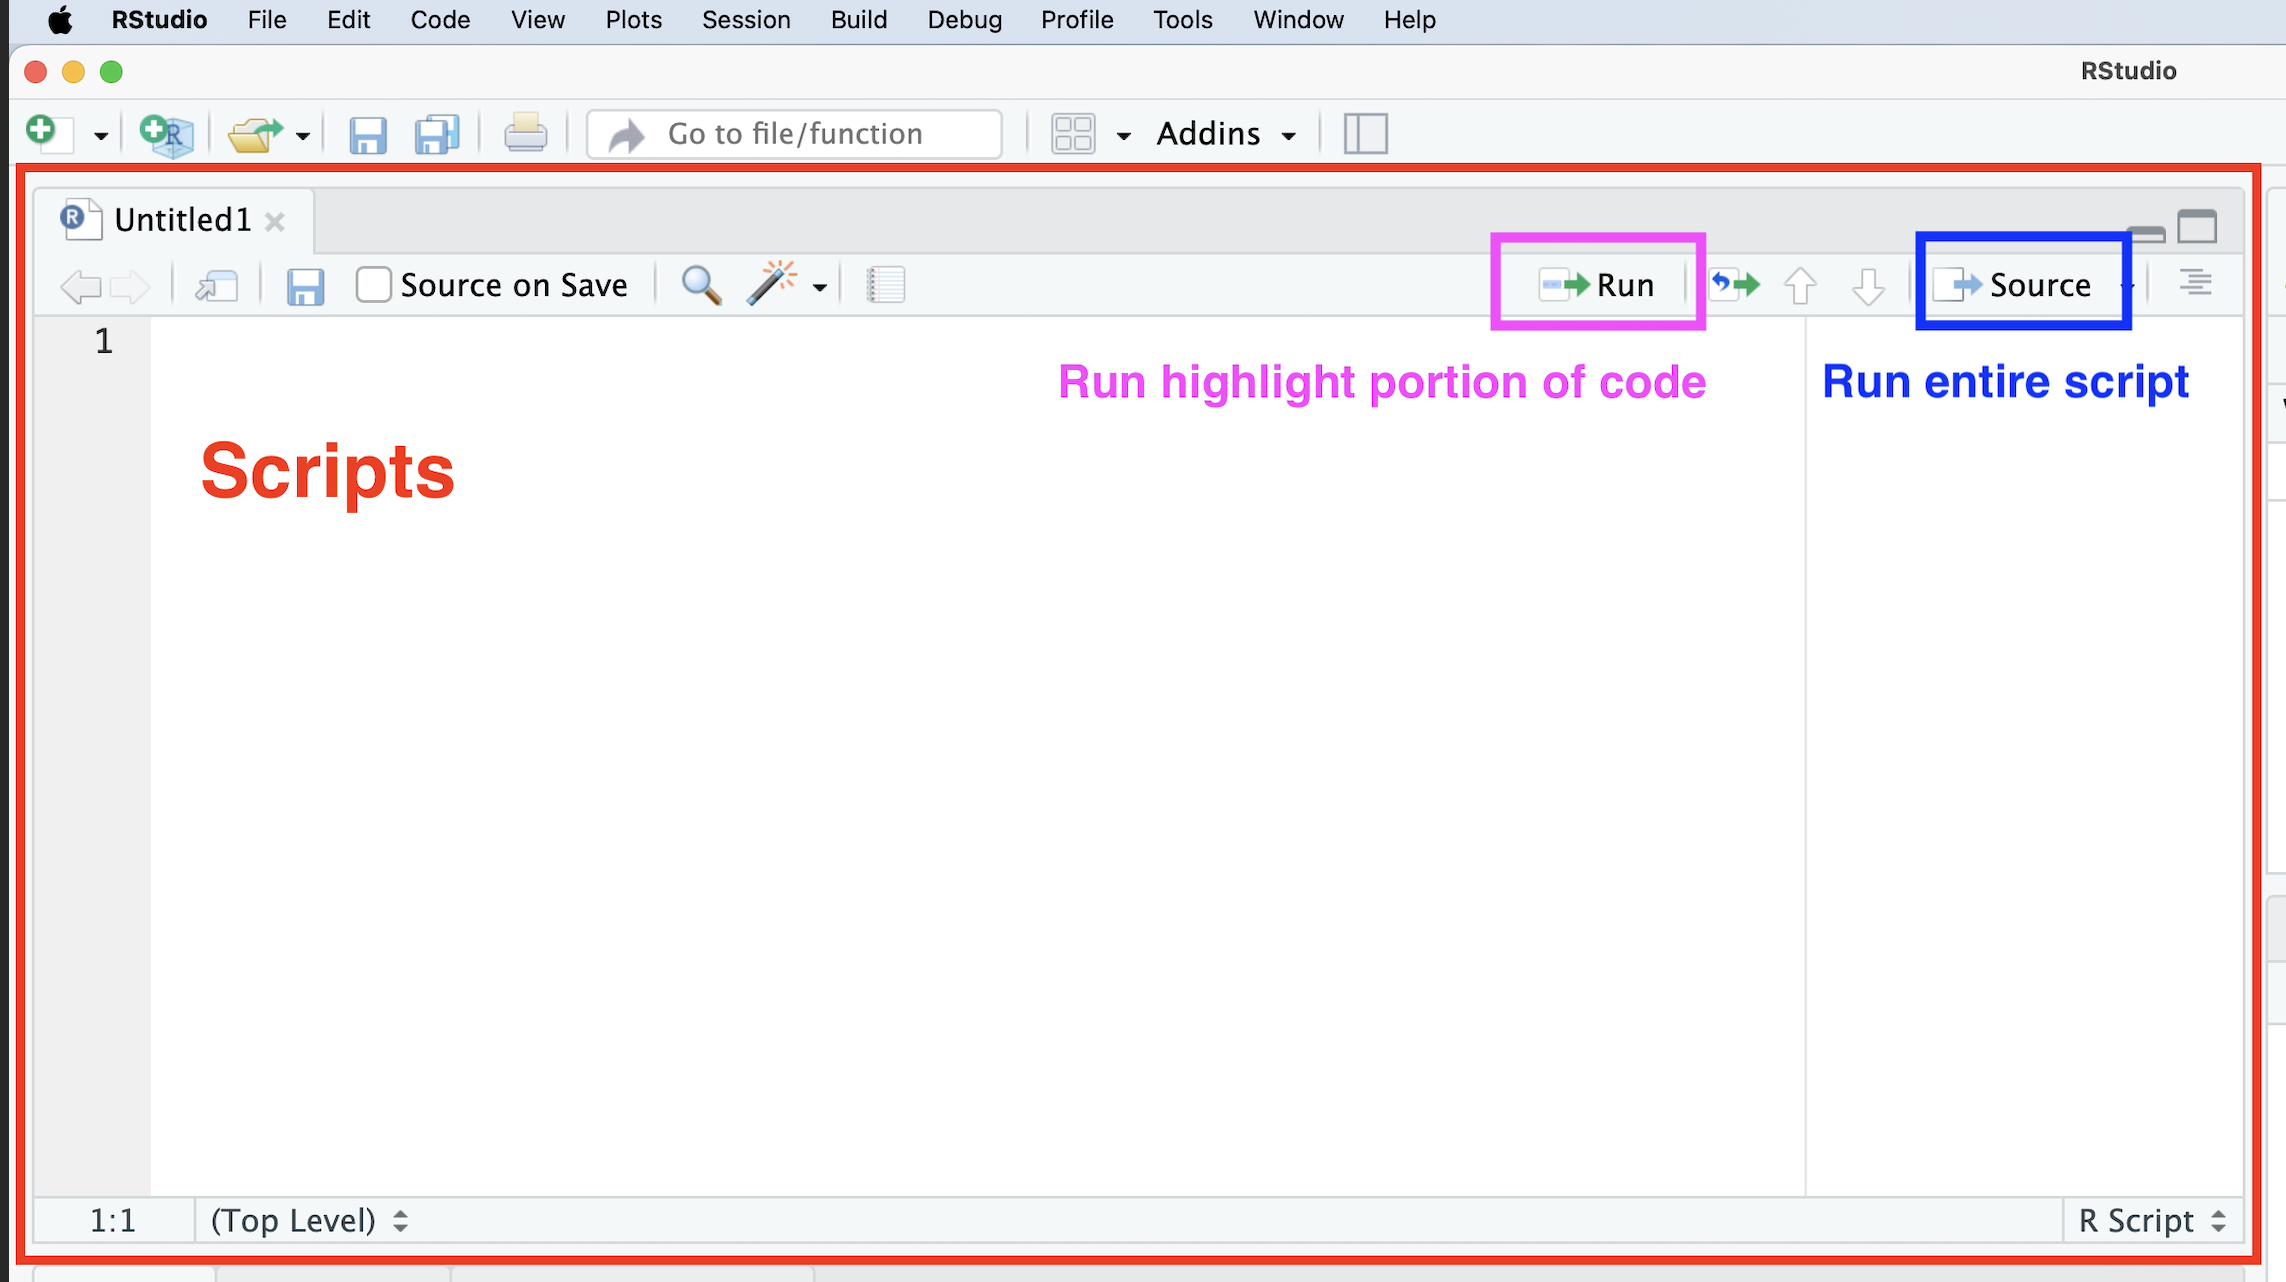
\includegraphics[width=1\linewidth]{R_script2.png}
    \end{figure}
\end{frame}

\begin{frame}{How to run code in the script}
    How to run a command: \\
    \begin{itemize}
        \item Type the command in the script and type
        \begin{itemize}
        \item \fbox{\texttt{Ctrl}} \fbox{\texttt{Enter}} (Windows)
        \item \fbox{\texttt{Command}} \fbox{\texttt{Enter}} (macOS)
        \end{itemize}
    \end{itemize} 
\end{frame}

\begin{frame}{How to create a new R Script}
    File $\rightarrow$ New file $\rightarrow$ R Script
    \begin{figure}
      \centering
      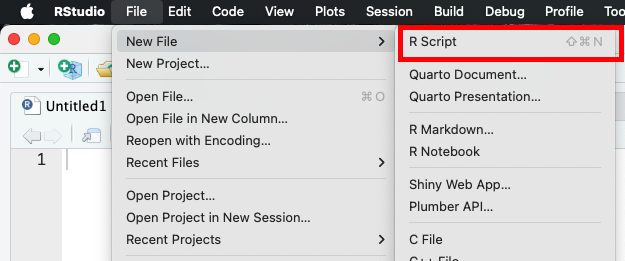
\includegraphics[width=1\linewidth]{截圖 2026-02-27 下午3.40.46.png}
    \end{figure}
\end{frame}


\begin{frame}{How to save a R Script}
    \begin{enumerate}
        \item Type
        \begin{itemize}
            \item \fbox{\texttt{Ctrl}} \fbox{\texttt{s}} (Windows)
            \item \fbox{\texttt{Command}} \fbox{\texttt{s}} (macOS)
        \end{itemize}
        \item Click the disk icon in the top left corner of the script window
        \begin{figure}
            \centering
            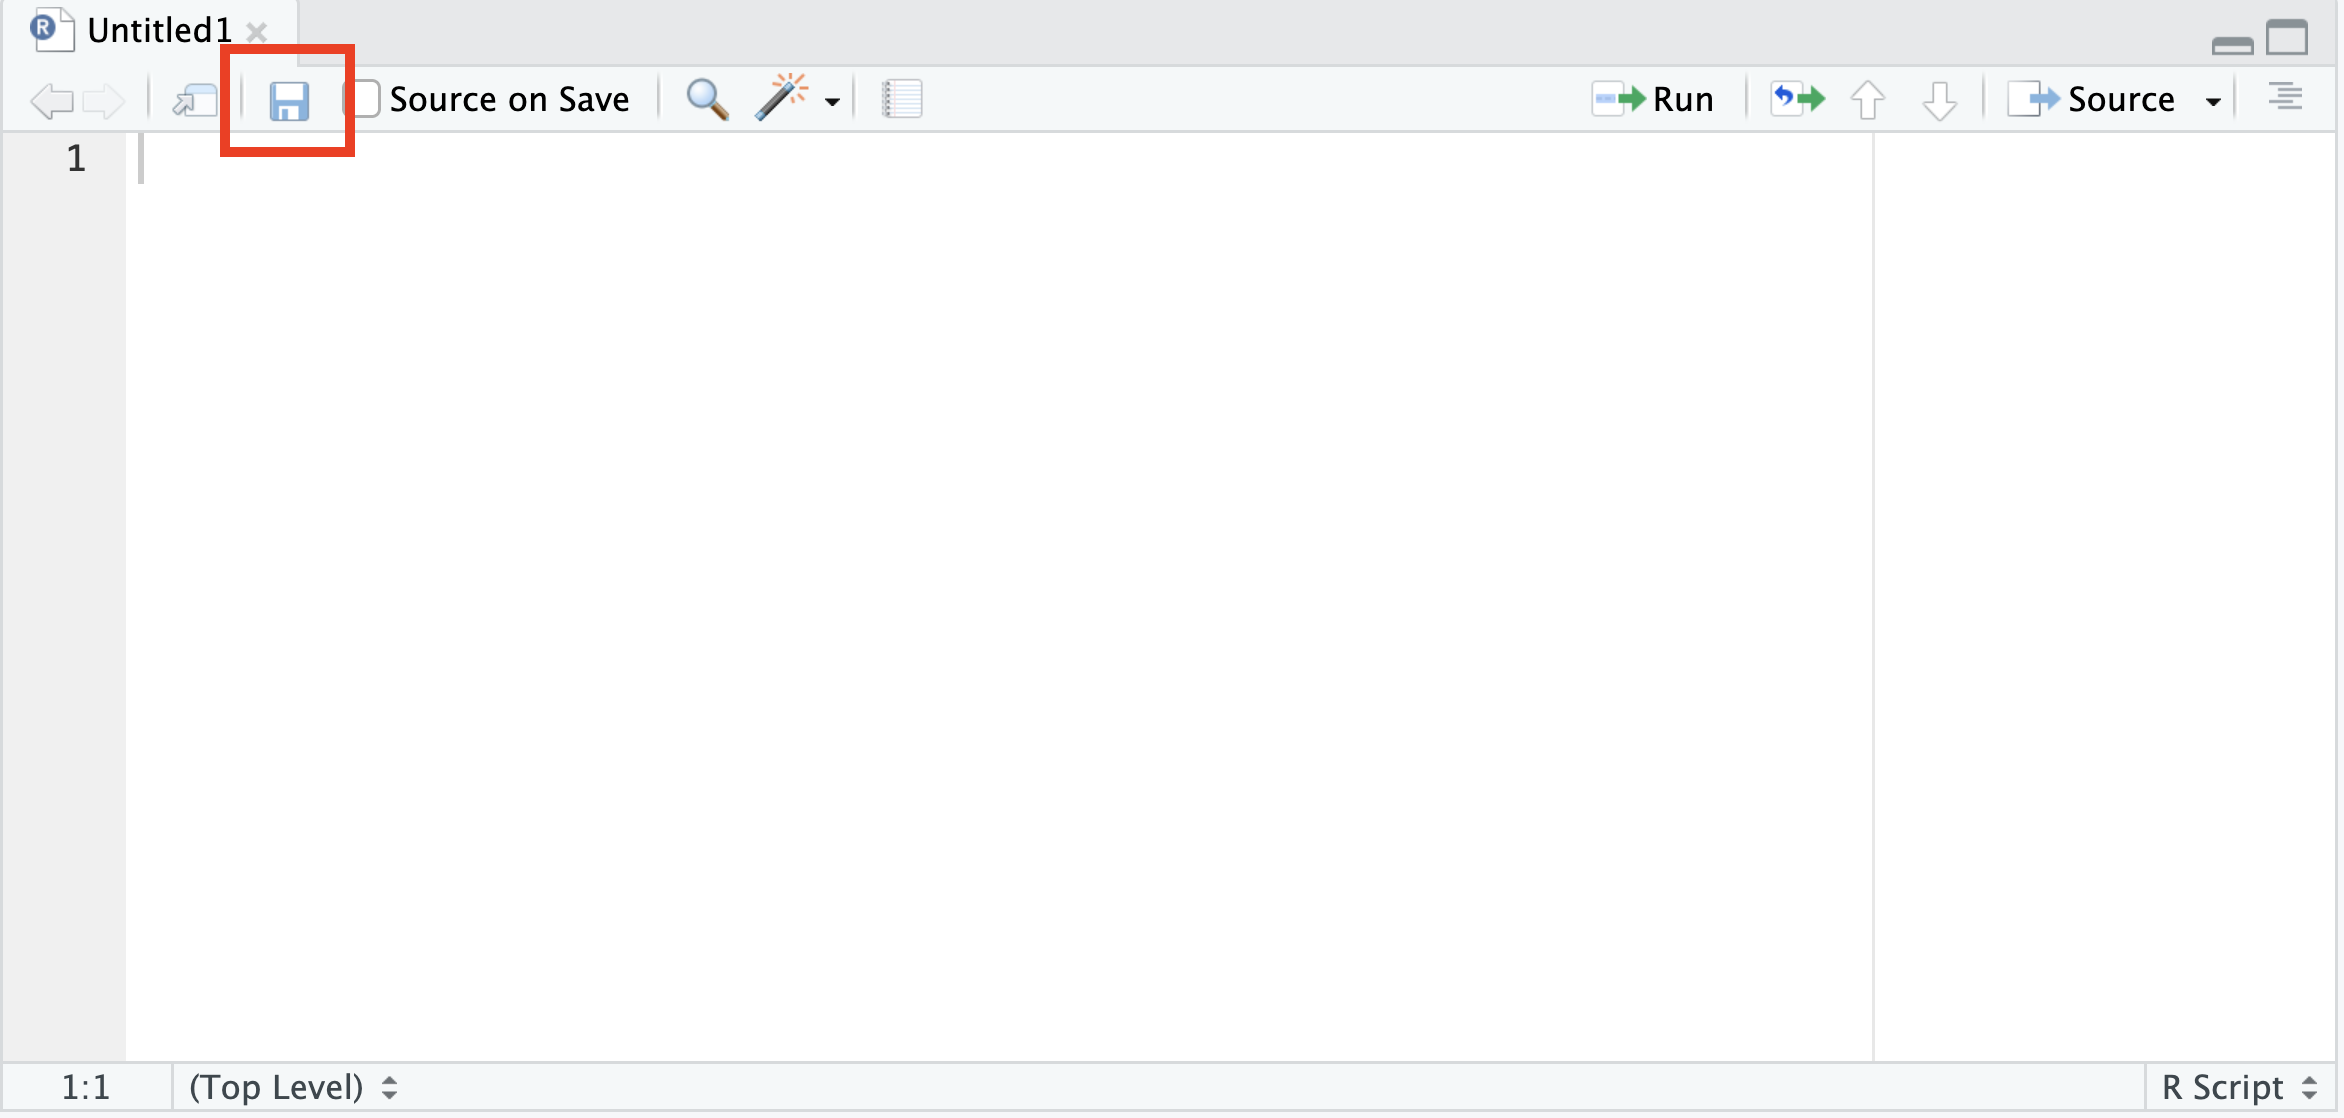
\includegraphics[width=1\linewidth]{R_script_save.png}
          \end{figure}
    \end{enumerate}


\end{frame}


\section{Practice}
\begin{frame}{Practice }

  Use R to calculate the following. \\
  Try assigning values to objects first, then perform the calculation

  \vspace{0.5em}

  \begin{enumerate}

    \item
    \[
      \frac{46\times628}{71}
    \]

    \item
    \[
      \ 7 \times (2^8 +56)
    \]

    \item
    \[
      \frac{log(|10-5|+1)+\sqrt{3^2+5^2}-e^{3-5}}{(3^3+5^3+1)}
    \]

  \end{enumerate}

\end{frame}



%%%%%%%%%%%%%%%%%%%%%%%%%%%%%%%%%%%%%%%%%%%%%%%%%%%%%%%%%%



\end{document}
